\documentclass[9pt,twocolumn,twoside]{rilabRxiv}
% Use the documentclass option 'lineno' to view line numbers
\setlength{\marginparwidth}{2cm}
\usepackage[textsize=tiny,colorinlistoftodos]{todonotes} % comments in margins
\definecolor{cornflowerblue}{rgb}{0.39, 0.58, 0.93}
\usepackage{multicol}


%%%%%%%Add comments in color
\newcommand{\ms}[1]{{\small \textcolor{green}{#1}}}
\newcommand{\jri}[1]{{\small \textcolor{red}{#1}}}
\newcommand{\citex}[1]{{\small \textcolor{red}{CITE(#1)}}}
\newcommand{\X}{{\textcolor{red}{X}}}

\newcolumntype{b}{X}
\newcolumntype{s}{>{\hsize=.5\hsize}X}

% Set supplement numbers to S and start counting newly
\newcommand{\beginsupplement}{%
        \setcounter{table}{0}
        \renewcommand{\thetable}{S\arabic{table}}%
        \setcounter{figure}{0}
        \renewcommand{\thefigure}{S\arabic{figure}}%
     }


\usepackage{hyperref}

\title{The chronology of linked selection in nonequilibrium populations}

\author[$\S$,a]{Raul Torres}
\author[$\ast$,a]{Markus Stetter}
\author[$\dagger$,1]{Ryan Hernandez}
\author[$\ddagger$,1]{Jeffrey Ross-Ibarra}

\affil[$\S$]{Biomedical Sciences Graduate Program, University of California San Francisco, San Francisco, CA, USA}
\affil[$\ast$]{Botanical institute, University of Cologne, Cologne, Germany}
\affil[$\dagger$]{Genome Quebec Innovation Center, McGill University, Montreal, Canada}
\affil[$\ddagger$]{Dept. of Evolution and Ecology, Genome Center, and Center for Population Biology, University of California, Davis, CA, USA}

\keywords{demography, background selection, linked selection}

\runningtitle{Demography and background selection} % For use in the footer

%% For the footnote.
%% Give the last name of the first author if only one author;
% \runningauthor{FirstAuthorLastname}
%% last names of both authors if there are two authors;
% \runningauthor{FirstAuthorLastname and SecondAuthorLastname}
%% last name of the first author followed by et al, if more than two authors.
\runningauthor{Torres, Stetter \textit{et al.}}


%%% Abstract %%%%%%%%%%%%%%%%%%
\begin{abstract}
Neutral genetic diversity across the genome is determined by the complex interplay of mutation, demographic history, and natural selection. While the direct action of natural selection is limited to functional loci across the genome, its impact can have effects on nearby neutral loci due to genetic linkage. These effects of selection at linked sites, referred to as genetic hitchhiking and background selection (BGS), are pervasive across natural populations. However, only recently has there been a focus on the joint consequences of demography and selection at linked sites, and empirical studies have sometimes come to apparently contradictory conclusions. In order to understand the relationship between demography and linked selection, we conducted an extensive forward simulation study of BGS under a range of demographic models. We found that levels of diversity compared to an equilibrium population vary  over time, and that the initial dynamics after a population size change are often in the opposite direction of the long-term expected trajectory. Our detailed observations of the temporal dynamics of neutral diversity in the context of selection at linked sites in nonequilibrium populations provides new intuition about why patterns of diversity under BGS vary through time in natural populations and helps reconcile previously contradictory observations.
Most notably, our results highlight that classical models of BGS are poorly suited for predicting diversity in nonequilibrium populations.
\end{abstract}
%%%%%%%%%%%%%%%%%%%%%%%%%%

\setboolean{displaycopyright}{false}

\begin{document}
\begin{multicols}{1}
\maketitle
\end{multicols}
\thispagestyle{firststyle}
%\firstpagefootnote
\correspondingauthoraffiliation{
Dept. of Evolution and Ecology, University of California, Davis, CA, USA
E-mail: rossibarra@ucdavis.edu \\
Genome Quebec Innovation Center, McGill University, Montreal, Canada
E-mail: ryan@McGill.edu\\
\textsuperscript{a} co-first authors
}
\vspace{-11pt}%


\section{Introduction}
\lettrine[lines=2]{\color{color2}T}{}
he effects of natural selection and demography on neutral genetic diversity within populations have long been of interest in evolutionary and population genetics.
Recent efforts in sequencing tens of thousands of genomes across a multitude of species have yielded new and valuable insights into how these two forces of evolution have shaped extant patterns of genomic variation.
Yet, while the theoretical underpinnings of the effects of natural selection and demography on genetic diversity have been investigated for decades \citep{smith1974hitch, nei1975bottleneck, maruyama1984population, maruyama1985population, kaplan1989hitchhiking, charlesworth1993effect, nordborg1996effect, hudson1995deleterious, tajima1989effect}, detailed investigation into how they jointly act to create patterns of diversity in different populations remains lacking.

Both theory and empirical observation have long shown that patterns of neutral genetic variation can vary regionally across the genome as a function of recombination rate \citep{smith1974hitch, begun1992levels}.
This is because natural selection operating on selected sites not only decreases genetic variation at the focal site but can also lead to decreases in nearby neutral genetic diversity due to genetic linkage \citep{cutter2013genomic}.
These effects, known as genetic hitchhiking \citep{smith1974hitch} (in which neutral variants rise to high frequency with adaptive variants) and background selection \citep{charlesworth1993effect} (BGS; in which neutral variants are removed along with deleterious variants) can be widespread across the genome.
Evidence for selection at linked sites has been found across an array of species, including \textit{Drosophila melanogaster} \citep{begun1992levels, comeron2014background, charlesworth1996background, andolfatto2007hitchhiking, sella2009pervasive, elyashiv2016genomic}, mice \citep{keightley2018understanding}, wild and domesticated rice \citep{flowers2011natural, xu2012resequencing}, \textit{Capsella} \citep{williamson2014evidence}, monkeyflowers \citep{stankowski2018tempo}, maize \citep{beissinger2016recent}, and humans \citep{sabeti2002detecting, reed2005fitting, voight2006map, mcvicker2009widespread, cai2009pervasive, hernandez2011classic, lohmueller2011natural}.

Demographic change can also impact patterns of diversity across the genome.
For example, neutral theory predicts that the amount of genetic diversity is proportional to a population’s effective population size (\textit{$N_e$}), such that changes in \textit{$N_e$} should result in concomitant changes to diversity \citep{kimura1983neutral}.
However, evidence suggests that such diversity also varies much less in magnitude across species when compared to their census population sizes \citep{lewontin1974genetic, leffler2012revisiting}.
One of the most common forms of a population size change is a population bottleneck, whereby populations suffer a large decrease followed by an expansion.
Bottlenecks can occur via domestication events \citep{doebley2006molecular, tang2010domestication, wiener2011deciphering, gaut2018demography}, seasonal or cyclical fluctuations in population size \citep{elton1924periodic, ives1970further, itoh2009seasonal, noren2014genetic}, and founder events \citep{david1988genetic, dlugosch2008founding, henn2012great}.
Notably, while the rate of loss of diversity in response to a population contraction is quite fast, the recovery of diversity following a population increase can be quite slow \citep{charlesworth2009effective}.
As a result, large contemporary populations may still yield patterns of low average genetic diversity if their population size was much smaller in the recent past.
In humans, this is clearly evident in European and Asian populations due to the out-of-Africa bottleneck \citep{10002015global}.

Because selection at linked sites and demography are both pervasive forces across a multitude of species, the characterization of how these two forces interact with one another is necessary in order to develop a full picture on the determinants of neutral genetic diversity.
The efficiency of natural selection scales proportionally with \textit{$N_e$} and the impact of selection at linked sites on neutral diversity is likely to be greater in larger populations and lower in smaller populations \citep{kaplan1989hitchhiking, cutter2013genomic, corbett2015natural}, although the rate of change for lowered diversity may diminish as populations reach larger and larger sizes \citep{gillespie2001population, santiago2016joint}.
Further, demographic changes can also increase (in the case of bottlenecks) or decrease (in the case of expansions) the rate of drift.
It is therefore plausible that the rate at which diversity at a neutral locus is perturbed by selection at linked sites could be highly dependent on both the current as well as long-term $N_e$ of the population.
This competition between the strength of selection at linked sites (which increases with N) and genetic drift (which decreases with N) may be a key contributor to the limited range of diversity observed among species  despite much larger observed differences in census size \citep{gillespie2001population, corbett2015natural, santiago2016joint}.
However, selection at linked sites alone may not be sufficient to explain the observed discrepancy between observed diversity and census populations sizes \citep{coop2016does}, and the action of both demography and selection at linked sites in concert may provide a better model.

Many models of selection at linked sites were also formulated with the assumption that the population is large enough (or selection strong enough) such that mutation-selection balance is maintained \citep{charlesworth1993effect, zeng2013coalescent, nicolaisen2013distortions}.
However, non-equilibrium demographic change may break such assumptions and forces other than selection may drive patterns of variation in regions experiencing selection at linked sites.
For example, during the course of a population bottleneck, genetic drift may transiently dominate the effects of selection at many sites such that traditional models of selection will poorly predict patterns of genetic diversity.
But selection at linked sites may also exacerbate the impact of genetic drift, resulting in even greater losses than expected by the action of demography alone.
A recent review by \citet{comeron2017background} included a cursory investigation into the impact of demography on diversity in regions under BGS and suggested a dependency on demographic history.
Recent empirical work in maize and humans has also demonstrated a strong interaction between demography and selection at linked sites \citep{beissinger2016recent,torres2018human}.
But these papers also demonstrate the need for a deeper understanding of the interaction between demography and selection at linked sites, as the two studies come to opposing conclusions about the impact of population bottlenecks and expansion on patterns of diversity in regions affected by selection at linked sites.

In order to more fully explore the joint consequences of demography and selection at linked sites, in this study we conducted extensive simulations of different demographic models jointly with the effects of BGS.
We find that the time span removed from demographic events is critical for populations experiencing non-equilibrium demography and can yield contrasting patterns of diversity that reconciles apparently contradicting results  \citep{beissinger2016recent,torres2018human}.
Additionally, the sensitivity of genetic diversity to demography is dependent on the frequency of the alleles being measured, with rare variants experiencing more dynamic changes through time.

Our results demonstrate that traditional models of selection at linked sites may be poorly suited for predicting patterns of diversity for populations experiencing recent demographic change, and that the predicted forces of BGS become apparent only after populations begin to approach equilibrium.
Importantly, even simple intuition about the effect of selection at linked sites may lead to erroneous conclusions if populations are assumed to be at equilibrium.
These results should motivate further research into this area and support the use of models that incorporate the joint effects of both demography and selection at linked sites.

\section{Materials and Methods}
\label{sec:materials:methods}

\subsection{Simulation model}

We simulated a diploid and randomly mating population using fwdpy11 v1.2a (\href{https://github.com/molpopgen/fwdpy11}{\emph{https://github.com/molpopgen/fwdpy11}}), a Python package using the fwdpp library \citep{thornton2014c++}.
Selection parameters for simulating BGS followed those of \citet{torres2018human}, with deleterious variation occurring at 20\% of sites across a 2 Mb locus and the selection coefficient, \textit{s}, drawn from two distributions of fitness effects (DFE).
Specifically, 13\% of deleterious sites were drawn from a gamma distribution (parameters: mean = $\alpha/\beta$, variance = $\alpha/\beta^2$) parameterized $\Gamma(\alpha = 0.0415, \beta = 80.11)$ and seven percent from a distribution parameterized $\Gamma(\alpha = 0.184, \beta = 6.25)$.
These distributions mimic the DFEs inferred across non-coding and coding sites within the human genome \citep{torgerson2009evolutionary, boyko2008assessing}.
Fitness followed a purely additive model in which the fitness effect of an allele was 0, $0.5s$, and $s$ for homozygous ancestral, heterozygous, and homozygous derived genotypes, respectively.
Per base pair mutation and recombination rates also followed those of \citet{torres2018human} and were $1.66 \times 10^{-8}$ and $8.2 \times 10^{-10}$, respectively.
We also included a 200 kb neutral locus directly flanking the 2 Mb deleterious locus in order to observe the effects of BGS on neutral diversity.
For all simulations, we simulated a burn-in period for 10N generations with an initial population size of 20,000 individuals before simulating under 12 specific demographic models.
The demographic models included one demographic model of a constant sized population (model 1) and eleven non-equilibrium demographic models incorporating both bottlenecks and expansion (models 2-12; Figures \ref{supp:models1}-\ref{supp:models2}; Table \ref{table:params}).
For each demographic model, we also conducted an identical set of neutral simulations without BGS by simulating only the 200 kb neutral locus.
Each model scenario was simulated 5,000 times.

\subsection{Diversity statistics and bootstrapping}

After the burn-in period, we measured genetic diversity ($\pi$) and singleton density ($\xi$; the number of singletons observed within a locus) within 10 kb windows across the 200 kb neutral locus every 50 generations using a random sample of 400 chromosomes.
We measured $\pi$ and $\xi$ for each demographic model by taking the mean of these values across each set of 5,000 replicate simulations.
For neutral simulations, we annotated $\pi$ and $\xi$ as $\pi_0$ and $\xi_0$, respectively.
We took the ratio of these statistics (i.e., $\pi/\pi_0$ and $\xi/\xi_0$) in order to measure the relative impact of BGS within each demographic model.
We bootstrapped the diversity statistics by sampling with replication the 5,000 simulated replicates of each demographic model to generate a new set of 5,000 simulations, taking the mean of $\pi$ and $\xi$ across each new bootstrapped set.
We conducted 10,000 bootstrap iterations and generated confidence intervals from the middle 95\% of the resulting bootstrapped distribution.

\subsection{Calculations of expected BGS}

To calculate the predicted equilibrium $\pi/\pi_0$ given the instantaneous $N_e$ at each time point for each demographic model, we used equation 14 of \citet{nordborg1996effect}, but modified it accordingly to incorporate two gamma distributions of fitness effects.
Additionally, in order to properly model our simulations, we only calculated the effects of BGS on one side of the selected locus.
This resulted in the following modified equation:


\begin{eqnarray*}
\begin{aligned}
\frac{N_e}{N}\equiv\frac{\pi}{\pi_0}= \\
exp\left( -\frac{U_T}{2R}\int^{\infty}_C\frac{1}{s}\bigg\{\int_0^R\frac{dz}{[1+r(z)(1-s)/s]^2}\bigg\}\Gamma(s,\alpha_T,\beta_T)ds \right)\times \\
    exp\left( -\frac{U_B}{2R}\int^{\infty}_C\frac{1}{s}\bigg\{\int_0^R\frac{dz}{[1+r(z)(1-s)/s]^2}\bigg\}\Gamma(s,\alpha_B,\beta_B)ds \right)
    \end{aligned}
\end{eqnarray*}

Here, $R$ is the total length of the selected locus in bp, $U$ is the total deleterious mutation rate across the selected locus, $r(z)$ is the genetic map distance between a neutral site and a deleterious mutation, and $s$ is the selection coefficient of a deleterious mutation.
The left side of the equation models the effects of BGS according to the gamma DFE inferred by \citet{torgerson2009evolutionary} (represented by $\Gamma(s,\alpha_T,\beta_T)$) and the right side of the equation models the effects of BGS according to the gamma DFE inferred by \citet{boyko2008assessing} (represented by $\Gamma(s,\alpha_B,\beta_B)$).

Because $N_e$ is not explicitly included in this model of BGS, we followed previous work \citep{charlesworth2012role, comeron2014background} in truncating selection at some value $C$,
such that $C = \gamma/2N_e$ (represented in the integral $\int^{\infty}_C$).
Here, $C$ represents the minimum selection coefficient which is treated as deleterious for the model and $\gamma$ represents the population scaled selection coefficient ($\gamma = 2N_es$) that determines the value of $C$.
Thus, this step excludes effectively neutral mutations from the model that should not contribute to BGS.
This truncation step also affects the values used for $U$ in the above equation, resulting in specific values of $U$ for each DFE.
We simulated different population sizes under our BGS simulation model to see how well the modified Nordborg model fit populations of different $N_e$ for different values of $\gamma$ (Figure \ref{fig:nordborgsims}).
We used a $\gamma = 0.15$ because this provided the best estimate of $\pi/\pi_0$ for the starting $N_e$ of our demographic models (i.e., $N_e = 20,000$).
While this value provides a coarse estimate for the effects of BGS on $\pi/\pi_0$ for a particular $N_e$, it will overestimate the effects of BGS for smaller $N_e$ (Figure \ref{fig:nordborgsims}).

%%%%%%%%%%%%%%%%%%%%%%%%%%%%%%%%%%%%%%%%%%%%%%%%%%%%%%
\section{Results}
%%%%%%%%%%%%%%%%%%%%%%%%%%%%%%%%%%%%%%%%%%%%%%%%%%%%%%

\subsection{Background selection under instantaneous population size change}

We first present the joint effects of demography and background selection (hereafter, BGS) under simple demographic models with a single instantaneous change in size (models 2-4; Figure \ref{fig:S1}).
While our simulations incorporated a 200 kb neutral region, we first focused on patterns of diversity generated within the 10 kb window nearest to the 2 Mb locus experiencing purifying selection, as this is where BGS is strongest.
Doing so allowed us to observe any change in the dynamics of $\pi$ and $\xi$ as they approached new population equilibria resulting from a change in size.
In the simple bottleneck models (models 2-3) we observed the expected strong decrease in $\xi$ and $\pi$ following  population contraction in both models of BGS and neutrality (Figure \ref{fig:S6}).
Similarly, we observed the expected rapid increase in $\xi$ compared to $\pi$ in our model of a simple population expansion (model 4; Figure \ref{fig:S6}).
In all cases values of $\xi$ and $\pi$ were lower in models with BGS and diversity values changed more rapidly than in the neutral case (Figure \ref{fig:S9}).

\begin{figure}[]
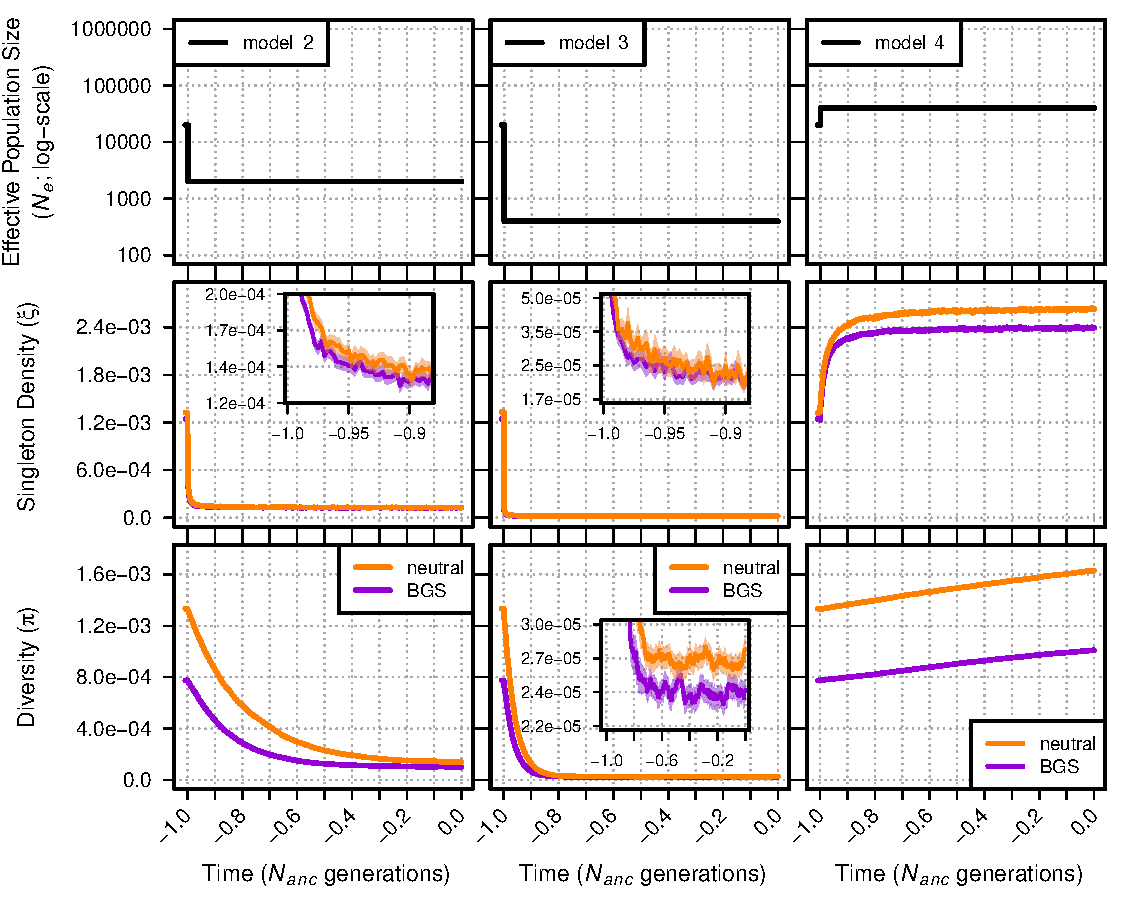
\includegraphics[width=\linewidth]{figures/FigS6.pdf}
\caption{Singleton density ($\xi$ per site) and diversity ($\pi$ per site) for models 2-4.
The top panel shows each demographic model; time proceeds forward from left to right and is scaled by the $N_e$ of the population at the initial generation ($N_{anc}$).
Diverstiy statistics are shown for neutral simulations (orange lines) and simulations with BGS (violet lines).
Insets show diversity using a log scale for improved detail.
Envelopes are 95\% CIs calculated from 10,000 bootstraps of the original simulation data.}
\label{fig:S6}
\end{figure}

To examine the interaction of demography and selection observed in empirical data \citep{beissinger2016recent,torres2018human}, we normalize $\pi$ and $\xi$ in models of BGS by their equivalent statistics generated under the same demographic model in the absence of any selection ($\pi_0$ and $\xi_0$).
We observed that $\pi/\pi_0$ and $\xi/\xi_0$ were dynamic through time in response to demography, with changes occurring to both their magnitude and direction (Figure \ref{fig:1}).
Moreover, changes to $\xi/\xi_0$ occurred more rapidly through time compared to $\pi/\pi_0$.
For example, in model 2 we observed a dip and rise in the $\xi/\xi_0$ statistic relative to equilibrium (model 1) within the first $\approx 0.1N_{anc}$ generations ($N_{anc}$ refers to the $N_e$ of the ancestral population prior to any demographic change).
Yet, for the same model, $\pi/\pi_0$ remained depressed for over $0.5N_{anc}$ generations (Figure \ref{fig:1}).
Similar patterns were observed for model 3, which experienced a greater reduction in size, although the pattern is less clear because of the greater sampling variance of $\xi/\xi_0$ due to the overall lower number of singletons.
In both population contraction models  $\pi/\pi_0$ and $\xi/\xi_0$ appeared to plateau at levels above that of model the equilibrium model.
In contrast, we observed markedly different dynamics in our model of simple population expansion (model 4), with a sustained increase in $\pi/\pi_0$ but only a transient increase in $\xi/\xi_0$ within the first $\approx 0.1N_{anc}$, followed by a reduction to levels below that of the equilibrium model.

\begin{figure}[]
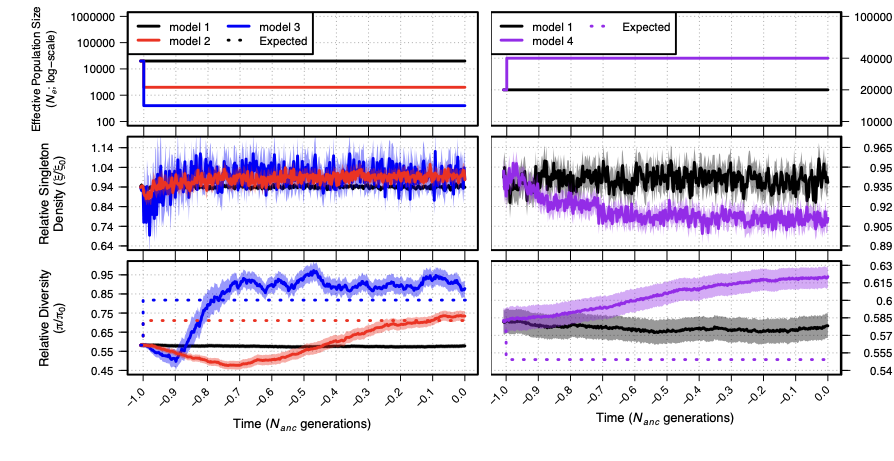
\includegraphics[width=\linewidth]{figures/tempF1.png}
\caption{Relative singleton density ($\xi/\xi_0$) and relative diversity ($\pi/\pi_0$) across time for demographic models 1-4.
The top panel shows each demographic model as in Figure \ref{fig:1}.
Black lines show $\xi/\xi_0$ and $\pi/\pi_0$ from simulations of a constant sized population (model 1).
Dotted lines in the bottom panel show the equilibrium  expectation of $\pi/\pi_0$ from  \citet{nordborg1996effect} given the specific selection parameters and the instantaneous $N_e$ at each time point.
Envelopes are 95\% CIs calculated from 10,000 bootstraps of the original simulation data.}
\label{fig:1}
\end{figure}

Changes in population size should lead to changes in the rate of genetic drift and the efficacy of natural selection and, thus, changes in the magnitude of BGS over time.
Indeed, under equilibrium contions, the classic model of BGS \citep{nordborg1996effect} predicts weaker BGS (with higher $\pi/\pi_0$) for smaller populations and stronger BGS (with lower $\pi/\pi_0$) for larger populations.
To compare these prediction to those of our simple demographic models, we calculated the predicted equilibrium $\pi/\pi_0$ under the classic model given the instantaneous $N_e$ at each generation.
In all three simple demographic models we observed that changes in $\pi/\pi_0$ over the short term differed qualitatively from the classic model  (Figure \ref{fig:1}; bottom panel).
The classic model predicts a higher value for $\pi/\pi_0$ in a smaller population, yet we observed a transient drop in $\pi/\pi_0$ directly after a contraction (models 2 and 3).
Similarly, while the classic model predicts a decrease in $\pi/\pi_0$ in larger populations, we observed an increase in $\pi/\pi_0$ with population expansion (model 4).
The trajectory of $\pi/\pi_0$ changed in our bottleneck models, eventually approaching the expectation predicted by the classic model, while $\pi/\pi_0$ in the expansion model continued to increase over the entire course of the simulation.

\subsection{Background selection under bottleneck-expansion models}

We built upon the simple two epoch demographic models  to test more complex  scenarios and better understand the relative effects of different events on patterns of diversity under BGS.
Specifically,  we simulated a population undergoing a contraction similar in size to models 2 and 3, but with a subsequent expansion to 400,000 individuals by the final generation (Figure \ref{fig:S2}.
These bottleneck-expansion models included both ancient ($1.0N_{anc}$ generations in the past, models 5-8) and recent ($0.1N_{anc}$ generations in the past, models 9-12) bottlenecks as well as both instantaneous expansion (models 5-6,9-10) or a sustained bottleneck (models 7-8,11-12).
These models recapitulated several patterns observed in our simple bottleneck models, but with added dynamics.
In all cases, diversity  in models with BGS was both lower (Figures \ref{fig:S4}-\ref{fig:S5}) and changed more rapidly (Figures \ref{fig:S7}-\ref{fig:S8}) than in neutral simulations.
Changes in diversity also occurred more quickly in models with a stronger or sustained bottleneck, and  $\xi$ again exhibited more rapid dynamics than did $\pi$.
Mirroring results from our simple bottleneck scenarios, models with an ancient bottleneck (models 5-8) showed a transient decrease in $\xi/\xi_0$ and $\pi/\pi_0$ followed by an increase to higher values (Figure \ref{fig:3new}).
Again changes in $\pi/\pi_0$ contrast with the expectations of the classic model, where  BGS is expected to become more efficient in larger populations, resulting in an expected decrease in $\pi/\pi_0$ (Figure \ref{fig:3new}, dotted line).
But while both $\pi/\pi_0$ and $\xi/\xi_0$ remain elevated in our simple bottleneck models, $\xi/\xi_0$ in these bottleneck and expansion models changes direction again and begins to decline, eventually reaching values below that of the equilibrium population.
Though the trajectories of $\pi/\pi_0$ and $\xi/\xi_0$ were truncated for models in which the bottleneck occurred in the recent ($0.1N_{anc}$ generations) past, they nonetheless appeared to behave qualitatively similar to ancient bottleneck models (Figure \ref{fig:S912}).

\begin{figure}[]
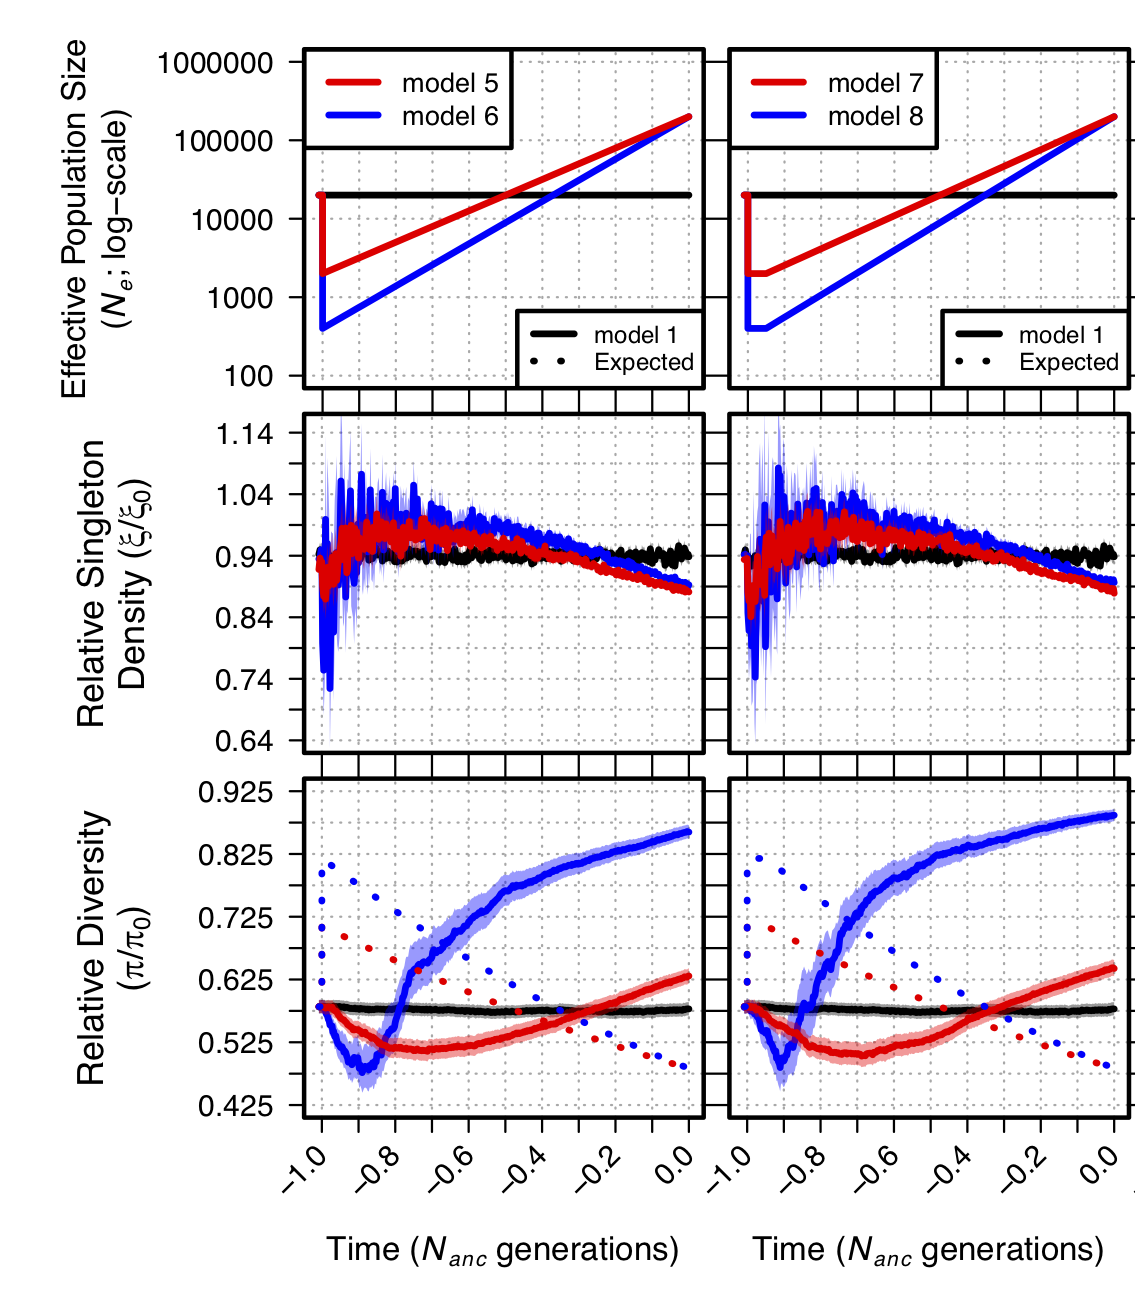
\includegraphics[width=\linewidth]{figures/fig3new.png}
\caption{Relative singleton density ($\xi/\xi_0$) and relative diversity ($\pi/\pi_0$) across time for demographic models 1 and 5-8.
The top panel shows each demographic model as in Figure \ref{fig:1}.
Black lines show $\xi/\xi_0$ and $\pi/\pi_0$ from simulations of a constant sized population (model 1).
Dotted lines in the bottom panel show the equilibrium  expectation of $\pi/\pi_0$ from  \citet{nordborg1996effect} given the specific selection parameters and the instantaneous $N_e$ at each time point.
Envelopes are 95\% CIs calculated from 10,000 bootstraps of the original simulation data.}
\label{fig:3new}
\end{figure}

\subsection{Patterns of diversity across the 200 kb neutral region}

We also measured patterns of $\pi/\pi_0$ across time for the entire 200 kb neutral region.
Doing so showed the characteristic ``trough'' structure of increasing relative diversity as a function of genetic distance from the focal locus under selection (model 5 shown in  \ref{fig:200kb}, see Figure \ref{fig:S912} for all models).
Change in $\pi/\pi_0$ over time generally followed patterns observed in the neutral window closest to the selected region.
In all of our ancient bottleneck models (models 2-8), for example, we see a decline in $\pi/\pi_0$ across the entire region followed by an increase to levels higher than in the ancestral population, while for recent bottlenecks (models 9-12) we see a consistent decline with no recovery and in our simple expansion model (model 4) $\pi/\pi_0$ increases monotonically through time.

Yet these general patterns obscure more subtle changes in the slope of $\pi/\pi_0$ with increasing distance from the selected region.
In models with a stronger bottleneck (models 2,3,6 and 8), where we expect the efficacy of selection to be most impacted, we see that the slope $\pi/\pi_0$ flattens over time, completely erasing the trough of diversity in the most extreme cases without recovery (models 2-3). 


\begin{figure}[]
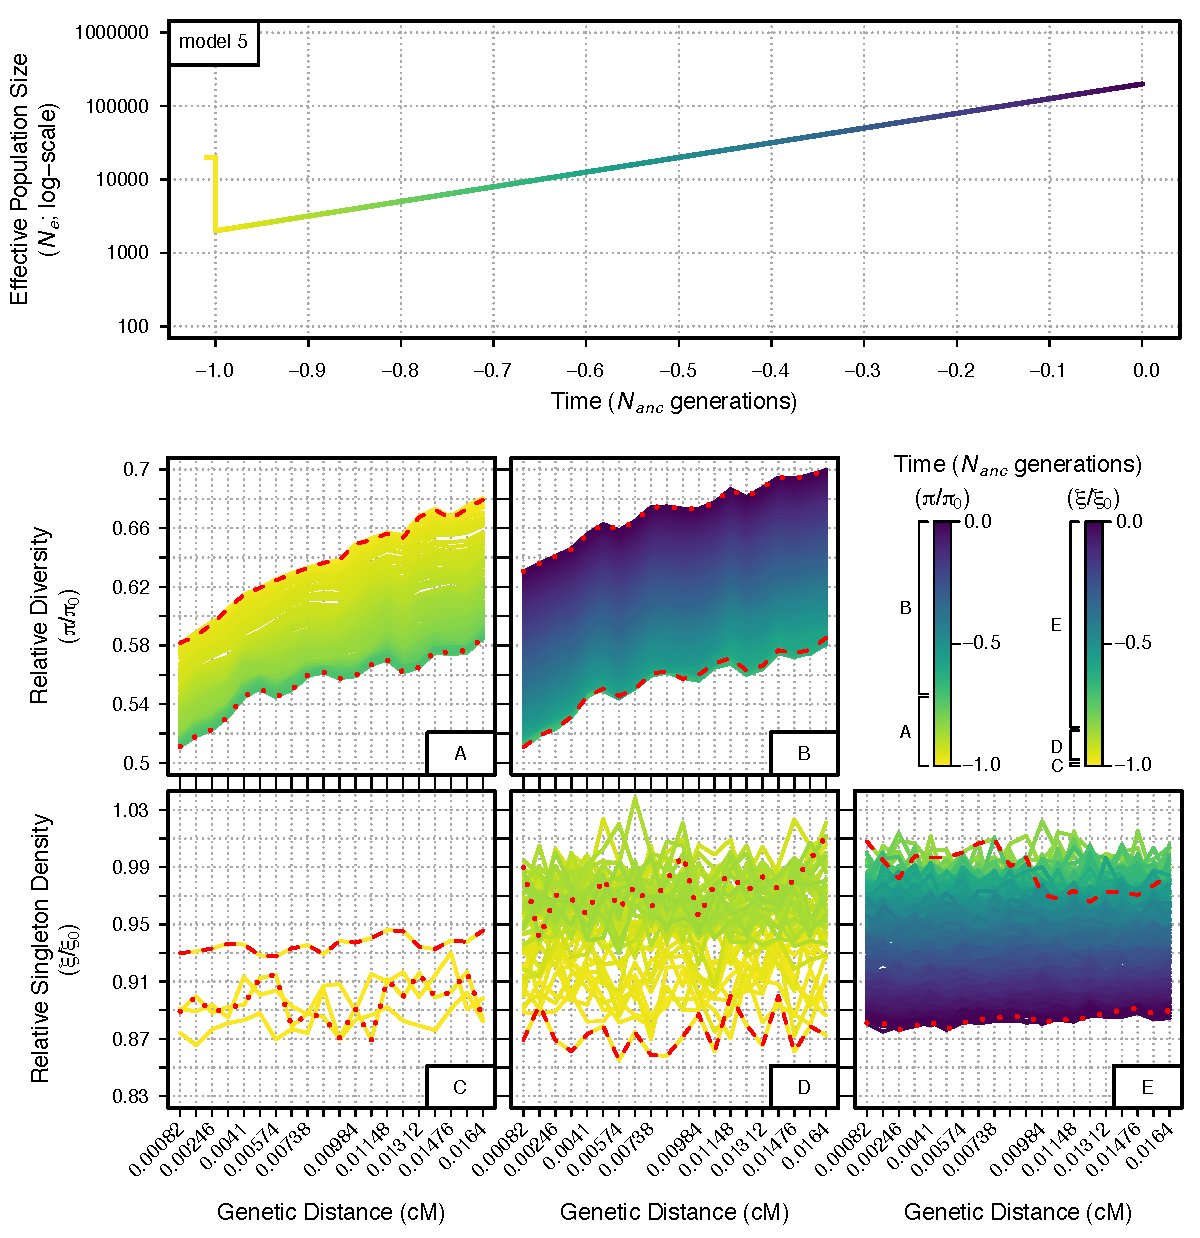
\includegraphics[width=\linewidth]{figures/FigS13.pdf}
\caption{Relative diversity ($\pi/\pi_0$) and singleton density ($\xi/\xi_0$) through time for demographic model 5 measured across a neutral 200 kb region under the effects of BGS.
The genetic distance of each 10 kb bin from the selected locus is indicated on the x-axis.
Each line measuring $\pi/\pi_0$ and $\xi/\xi_0$ represents one of the 401 discrete generations sampled from the demographic model; colors follow the demographic model at the top (time is scaled as in Figure \ref{fig:s6}) and in the figure legend.
Multiple plots are given in order to prevent overlap of the measurements between generations (see legend for specific generations covered in each plot).
Blue dashed lines and red dashed lines indicate the first generation and last generation measured within each plot.}
\label{fig:200kb}
\end{figure}

Finally, while  $\xi/\xi_0$ across the regions also largely followed patterns seen in the neutral window proximal to the selected region, a closer look across the 200 kb regions yielded no clear patterns. 
Troughs were slightly apparent for the final generations of some models (models 5 and 7), but the stochasticity between windows for $\xi/\xi_0$ swamped any other patterns that might otherwise be evident.

%%%%%%%%%%%%%%%%%%%%%%%%%%%%%%%%%%%%%%%%%%%%%%%%%%%%%%
\section{Discussion}
%%%%%%%%%%%%%%%%%%%%%%%%%%%%%%%%%%%%%%%%%%%%%%%%%%%%%%

\subsection{General patterns of diversity}

%%% Response of diversity to demography \citex and BGS \citex in isolation reasonably well understood.
(explain)
We show here that neither of these explains well the combined action of both.

%%% In each of our models, the first effects we see are due to demography, and fit well with expectations.
(explain)
This is why we see it happen equally across the whole region initially 
While the effects of BGS should be attenuated in populations wd3ith lower $N_e$ (because the efficacy of purifying selection is weakened), the drop in $\pi/\pi_0$ instead demonstrated that the populations were dominated by the effects of allelic loss, which is expected for populations suffering a strong bottleneck.
Additionally, more rapid effects were observed for model 3s despite the fact that the expectation of $\pi/\pi_0$ for model 3 was actually higher than for model 2.
These observations made it clear that effects of BGS on $\pi/\pi_0$ immediately following a reduction in $N_e$ were not driven by a change in the efficacy of natural selection from population decline, but rather by the increased sensitivity of allelic loss within these regions -- with greater rates of loss accompanying greater reductions in population size.

%%% But effects happen faster for region under BGS.
Can think of this as Ne effect (better explanation?)
The diversity-reducing effects of BGS have often been modeled as a reduction in $N_e$ [56], which has been observed to increase sensitivity to drift for populations experiencing recent bottlenecks [51] (though we caution that effects of BGS on the SFS cannot be simplified to this extent [57]).
 Intuitively, these faster approaches to new equilibrium levels under BGS in response to size changes make sense if we consider the fact that the distance between initial and final equilibrium diversity levels for both $\pi$ and $\xi$ are closer to one another  under BGS when compared to neutrality (Figure S6; Table 2-3). 
This  provided a potential explanation for why we observed the specific dynamics of $\pi/\pi_0$ immediately following a size change.
This argument likely does not hold for model 4 because, due to itc higher $N_e$, it is unlikely that equilibrium has yet been reached. However, the observation of an increase in $\pi/\pi_0$ for model 4 did provide supporting evidence that a
 faster approach to equilibrium under BGS still existed under an
 expansion model. 
 Indeed, moderl 4 $\pi$ under BGS changed more quickly than
 under neutrality (Figure S9).
Observations of the dominant impact of genetic drift and weakened BGS
following a population reduction were also apparent when measuring
patterns of $\pi/\pi_0$ in models that had a more sustained
contraction (i.e., models 7 and 8). There, a decline in
$N_e$ was sustained for an additional 0.5
$N_{anc}$ generations before the expansion event began
(Figure S2). For these models, the rise of $\pi/\pi_0$
resulting from weakened BGS occurred more quickly than for their
counterpart models with an immediate expansion (Figure S3). For example,
the inflection point at which $\pi$ under BGS surpassed $\pi$ under neutrality
occurred at -0.305 and -0.848 $N_{anc}$ generations
for models 7 and 8, respectively (Figure S7). For models 5 and 6, these
inflection points occurred later in time at -0.235 and -0.785
$N_{anc}$ generations, respectively. Further, the
final $\pi/\pi_0$ values for models 7 and 8 were 0.643 and
0.887 but for models 5 and 6, they were only 0.631 and 0.860. Thus, the
sustained lower $N_e$ of models 7 and 8 aided in
accelerating the approach to the new equilibrium established by
population reduction. This provided further evidence for the dominant
role that population bottlenecks have for patterns of diversity under
BGS, even when populations expand past their ancestral size.

%%% After some time, however, the reduced efficacy of selection takes over. 
$\pi/\pi_0$ starts increasing for bnecks, decreasing for expansion
While general trends in diversity and comparisons to equilibrium theory highlight that the combined process of demography and linked selection is complex, data from a single window is insufficient to distinguish between the effects of these processes.
Surveying diversity across neutral windows varying in recombination distance from the selected region, however, provides some insight into the temporal and spatial impacts of both the direct and indirect effects of population size change. 

%%% Thus the effect seen depends on time since demography in units of N generations.

%%% Why not hit classical equilibrium. 
1) time 2) However, we note that this expectation underestimated $\pi/\pi_0$ for model 3 because the threshold of $s < 0.15/2N_e$ was likely not conservative enough to ignore deleterious mutations that behave neutrally under the low $N_e$ size of 400 for that model.


%%% Everything faster with $\xi$.
Each of these dynamics occurred more quickly for $\xi/\xi_0$, which was expected since approaches to equilibrium are more rapid for rare variants relative to common variants.
Thus, despite the demographic change resulting in immediate decreases to $\xi/\xi_0$ and $\pi/\pi_0$, patterns of relative diversity in populations suffering a contraction eventually approached their expected higher equilibrium values under weakened BGS, with rates dependent on the frequency of the alleles being observed and the  magnitude of the population reduction. 
This was evident from the fact that the final $\pi/\pi_0$ values for models 2 and 3 were
Since $\xi/\xi_0$ is already less affected (and, thus, closer to 1) than $\pi/\pi_0$ because BGS perturbs common frequency bins of the SFS more than rare ones [57], any signal using rare frequency bins will be inherently more difficult to capture across differing magnitudes of BGS. However, more extensive simulations may help to uncover such patterns.
Since $\xi/\xi_0$ is already less affected (and, thus, closer to 1) than $\pi/\pi_0$ because BGS perturbs common frequency
bins of the SFS more than rare ones [57], any signal using rare
frequency bins will be inherently more difficult to capture across
differing magnitudes of BGS. However, more extensive simulations may
help to uncover such patterns.


\subsection{Comparisons to empirical data}

One of the motivations for the work presented here is the fact that empirical analyses evaluating the impact of demography on linked selection have come to conflicting conclusions \citep{torres2018human, beissinger2016recent}.
Cultivated maize, for example, is thought to have undergone a bottleneck during the process of domestication \citep{eyre1998investigation,tenaillon2004selection,wright2005effects}, followed by a substantial expansion to a modern size several orders of magnitude larger than its wild ancestor teosinte \citep{beissinger2016recent, bellon2018evolutionary}.
A recent analysis of selection at linked sites in  maize and teosinte found differences, and interpreted them to be due to the timing of these demographic events.
\citet{beissinger2016recent} found that $\pi/\pi_0$ exhibited a greater trough around selected sites in teosinte, consistent with this taxon's larger long-term $N_e$.
However, their analysis of $\xi/\xi_0$ found the opposite pattern --- stronger effects in maize than teosinte --- a result the authors interpreted as a reflection of the post-domestication expansion and increased efficacy of selection in domesticated maize in the recent past.

Human demographic history appears at least qualitatively similar to that of maize, with a bottleneck associated with migration out of Africa followed by considerable recent population expansion \citep{tennessen2012evolution}.
In spite of this, however, analysis of linked selection in humans produced different results \citep{torres2018human}.
As in maize, the bottlenecked European population was found to have lower $\pi/\pi_0$ than African populations.
But unlike maize, the authors find similarly low values of $\xi/\xi_0$, and interpret both results as consistent with decreased efficacy of selection due to the out-of-Africa bottleneck.

While there are a number of challenges associated with accurate estimation of historical demography in empirical systems \citex{}, our models highlight the fact that  results seen in both maize and humans are plausible  under even relatively simple models broadly consistent with the dynamics of these two systems.
Under our model of bottleneck and expansion (Figure \ref{fig:3new}), for example, sampling in the present (generation 0) returns results similar to those seen in maize, with $\pi/\pi_0$ higher than a constant-size reference population but $\xi/\xi_0$ showing lower values due to the increased efficacy of selection in the expanding population.
Yet a sample taken anytime between generation -0.8 and -0.2 would reveal the observed pattern in humans, with both larger $\pi/\pi_0$ and $\xi/\xi_0$ still reflecting the impacts of the more recent bottleneck.

% TEXT HERE EXPLAINING




%%%%%%%%%%%%%%%%%%%%%%%%%%%%%%%%%%%%%%%%%%%%%%%%%%%%%%
\section{Here be dragons}
%%%%%%%%%%%%%%%%%%%%%%%%%%%%%%%%%%%%%%%%%%%%%%%%%%%%%%
%behavior of $\pi/\pi_0$ and $\xi/\xi_0$ in simple demographic models
%models2-3
%These patterns were made evident when observing the more rapid relative decrease in diversity in our selection models with BGS versus neutrality.
% When compared to their initial equilibrium starting points, $\pi$ under BGS suffered faster rates of loss compared to the neutral case for both models (Figure S9), with the fastest rates of loss accompanying larger reductions in $N_e$ (i.e., model 3).
%Importantly, these results demonstrated that classical models that predict the impact of BGS on $\pi/\pi_0$, such as the Nordborg model, implicitly assume an equilibrium population at  mutation-selection balance [58] and are inappropriate for predicting true patterns of genetic diversity for populations that have udnergone recent size changes.

%model4

%The more sensitive and rapid response to population increase under BGS
%recapitulated the faster approaches to equilibrium that were exhibited
%in the contraction models. Intuitively, these faster approaches to new
%equilibrium levels under BGS in response to size changes make sense if
%we consider the fact that the distance between initial and final
%equilibrium diversity levels for both $\pi$ and $\xi$ are closer to one another
%under BGS when compared to neutrality (Figure S6; Table 2-3). This
%provided a potential explanation for why we observed the specific
%dynamics of $\pi/\pi_0$ immediately following a size change.
%This argument likely does not hold for model 4 because, due to its
%higher $N_e$, it is unlikely that equilibrium has
%yet been reached. However, the observation of an increase in
%$\pi/\pi_0$ for model 4 did provide supporting evidence that a
%faster approach to equilibrium under BGS still existed under an
%expansion model. Indeed, moderl 4 $\pi$ under BGS changed more quickly than
%under neutrality (Figure S9). Presumably, this also indicates that $\pi$
%under BGS will reach a new equilibrium first, at which point
%$\pi/\pi_0$ will begin a downward trajectory in response to $\pi$
%continuing to increase under neutrality but $\pi$ under BGS remaining at a
%constant equilibrium. This is a likely outcome if the qualitative
%changes in $\xi/\xi_0$ foreshadow the future dynamics of
%$\pi/\pi_0$. The end result would also include a decrease in
%$\pi/\pi_0$ relative to its initial starting point, with
%$\pi/\pi_0$ eventually reaching a value close to its
%expectation (Figure 2; dotted lines). Although we foresee no reason why
%this prediction should not hold true, more extensive simulations will be
%necessary to confirm this.


relatively higher than its initial value (Figure S8). This caused the
elevated $\xi/\xi_0$ exhibited in the final generation of
models 9-12 (Figure S3).

Because the history of models 9-12 only lasted 0.1
$N_{anc}$ generations, we also observed much more
limited dynamics of $\pi/\pi_0$ and $\xi/\xi_0$.
Specifically, $\pi/\pi_0$ did not recover above its initial
starting point by the final generation and $\xi/\xi_0$ did not
decrease in response to the population expansion, but rather continued
to remain elevated (Figure S3). These features are important because
they demonstrated that qualitatively similar demographic events, such as
the bottleneck-expansion model shared by models 5-8 and 9-12, can yield
opposite trends in statistics used as proxies for measuring the
intensity of BGS. Thus, the resulting effects on patterns of relative
diversity under BGS depend on how far removed the point of observation
is from a particular demographic event. Such patterns also help to
reconcile the qualitatively different observations yielded by previous
studies [20,51] (discussed further below).


Recently, two empirical investigations into the joint impacts of
demography and selection at linked sites in the context of BGS yielded
interesting and intuitive, albeit contradictory, observations.
Beissinger et al. [20] conducted a study across 36 samples from
maize and its wild progenitor teosinte. They found that patterns of
relative genetic diversity (i.e., $\pi/\pi_0$) across regions
experiencing linked selection in maize, which underwent a demographic
bottleneck during domesticaiton, were higher than in teosinte. They
attributed this to the historically larger $N_e$ of
teosinte, which led to more efficient natural selection and thus a
greater impact of BGS on neutral diversity. However, the contemporary
population size of maize, a staple food crop grown world-wide, is now
much larger than teosinte and should be experiencing stronger selection
in its recent history. Supporting this hypothesis, relative singleton
density of neutral sites in maize, which should reveal more recent
signals of evolutionary history, was lower compared to teosinte.
However, Torres et al. 2018 [51] revealed opposite patterns in
humans. There, through a analysis of over 2,500 human genomes, they
observed that relative genetic diversity ($\pi/\pi_0$) was
lower in non-Africans, a population that has undergone a series of
extensive population bottlenecks and exhibits a low long-term
$N_e$, when compared to Africans. Additionally,
relative singleton density was also higher in non-Africans. In
conclusion, the authors attributed these patterns to a higher
sensitivity to demography and drift in regions of selection at linked
sites, thus yielding lower relative diversity in bottlenecked
populations. They also concluded that the greater long-term
$N_e$, and thus more effective purifying selection
and greater BGS, of Africans has led to their observed lower relative
singleton density.

While these patterns observed in maize and humans are seemingly in
disagreement, important demographic details, such as the length of the
population bottleneck and the time since the post-bottleneck population
expansion began, may also be significant contributors to these results.
As our simulations demonstrated, it is possible for two qualitatively
similar demographic histories to yield opposite patterns if the window
of time in which those patterns are observed are different. In the case
of maize compared to teosinte, observations are being made at a time in
which BGS is operating less effectively on removing average pairwise
diversity (due to its lower long-term $N_e$) but
more effectively on singletons (due to its higher contemporary
$N_e$). But if this population had been sampled more
closely to its population bottleneck event, observations of relative
diversity may have been more aligned with what is currently observed for
humans. The approximate number of generations removed from the
domestication bottleneck event for maize is about 15,000 generations
[20]. For humans, the approximate number of generations removed from
the out-of-Africa bottleneck event is only 6,000 generations [51].
Therefore, it is not unreasonable to suspect that these different
timespans contribute to the qualitatively different observations now
being observed.

Importantly, these two studies provide striking examples of the
importance of considering the impact of demography and time on extant
patterns of diversity to avoid mis-attributing the underlying forces
driving those patterns in regions experiencing selection at linked
sites. Since the null expectation of a natural population should be that
it is not at demographic equilibrium [59], alternative hypothesis
testing on selection at linked sites should also include the effects of
non-equilibrium demography and how they affect patterns though time.
However, in the specific context of maize and humans, we also note that
other details, such as the periodic bottlenecks suffered by non-Africans
(which may have further accelerated drift) and the differences among the
distribution of fitness effects for these two species, are equally
important to consider and warrant further investigation as well.

Recent model development incorporating demography into models of BGS
holds promise on generating demographically aware models on the effects
of selection at linked sites in populations. In particular, results from
Zeng 2013 [48], which formulated a simulation-based structured
coalescent model of BGS with demography, also showed that demography can
perturb levels of genetic diversity under BGS through time. In a
separate study, an analytical model which is capable of incorporating
changing demography was formulated and will prove more ideal for
performing inference of selection at linked sites in dynamic populations
[49]. Both of these models, though, are limited in their ability to
accurately predict the effects of selection at linked sites when
mutation-selection balance breaks down, which typically occurs when the
population scaled selection coefficient, $\gamma$, approaches 1. In
general, the deterministic approximation implicit for models of BGS may
not be suitable for $\gamma \leq 3$ [56]. During the course of a
bottleneck, as we have simulated here, $\gamma$ is likely to fall below
these thresholds and patterns of diversity may be more strongly affected
by other processes such as genetic drift or the ``interference
selection'' regime described in Good et al. 2014 [60]. For the case
in which $s$ is drawn from a skewed distribution, such as the gamma
distribution, the deterministic approximation is further likely to break
down when $s$ is small. We attempt to limit these specific issues
in the Nordborg model by simply truncating $s$ so that predictions
better match observed levels of BGS for various population sizes
(albeit, under the additional assumption of demographic equilibrium).
This simplistic approach may be suitable for other models of BGS, but as
our results showed, it will likely provide only a coarse estimate for
the prediction of diversity under BGS (Figure S21).

\hyperdef{}{ux5f30j0zll}{}{}Finally, our results extend the recent
debate on patterns of diversity in selected sites in non-equilibrium
populations (especially in humans [61--64]) to patterns of diversity
across neutral sites. For the specific case of selected sites, sites
under strong selection are more sensitive to demographic change and will
reach new equilibrium frequency levels more quickly than neutral sites
or weakly selected sites [65--67]. As we have shown here in the
context of neutral sites, because the underlying equilibrium frequency
of neutral sites depends on the strength of selection at linked sites,
demographic change will also result in distinct responses to their
change in frequency. In addition, the rate of change will also depend on
which bins of the SFS diversity is being measured with. Together, this
results in the complex change of $\pi/\pi_0$ and
$\xi/\xi_0$ through time that we observed from our simulations.
This insight should provide caution, however, for studies attempting to
uncover the action of natural selection by comparing sites within the
genome since, even when controlling for the strength of BGS itself,
frequencies of neutral sites may still be at different relative levels
depending on the recent demographic history of the population.



Thus, the
impact of population contractions on mitigating the effects of BGS
resulted in larger shifts of $\pi/\pi_0$ in regions of the
genome already under the strongest amount of BGS.
This makes sense since regions farther removed from loci under purifying selection (i.e., under weaker effects of BGS) have values of $\pi/\pi_0$ closer to the neutral expectation of 1.
Thus, the upper bound for change in $\pi/\pi_0$ will be more limited there compared to regions more
proximal to a selected locus.
This provided further evidence for the dominant effects of
drift and allelic loss on driving the initial decrease in
$\pi/\pi_0$ immediately following a population contraction,
which should have unbiased effects across all bins within the trough.
During the subsequent recovery to higher values of $\pi/\pi_0$, we saw smaller differences arise
between the nearest and farthest 10 kb bins, demonstrating the expected
weakening effects of BGS following a population decline. This weakening
of the trough structure was also most apparent for model 3, with
patterns of $\pi/\pi_0$ appearing essentially flat across the
200 kb region in the final generation (Figure S11).

\section{Acknowledgments}


\bibliography{example-bibliography}

%\pagebreak
\onecolumn

\beginsupplement
\section*{Supplement}

\begin{figure*}[h!]
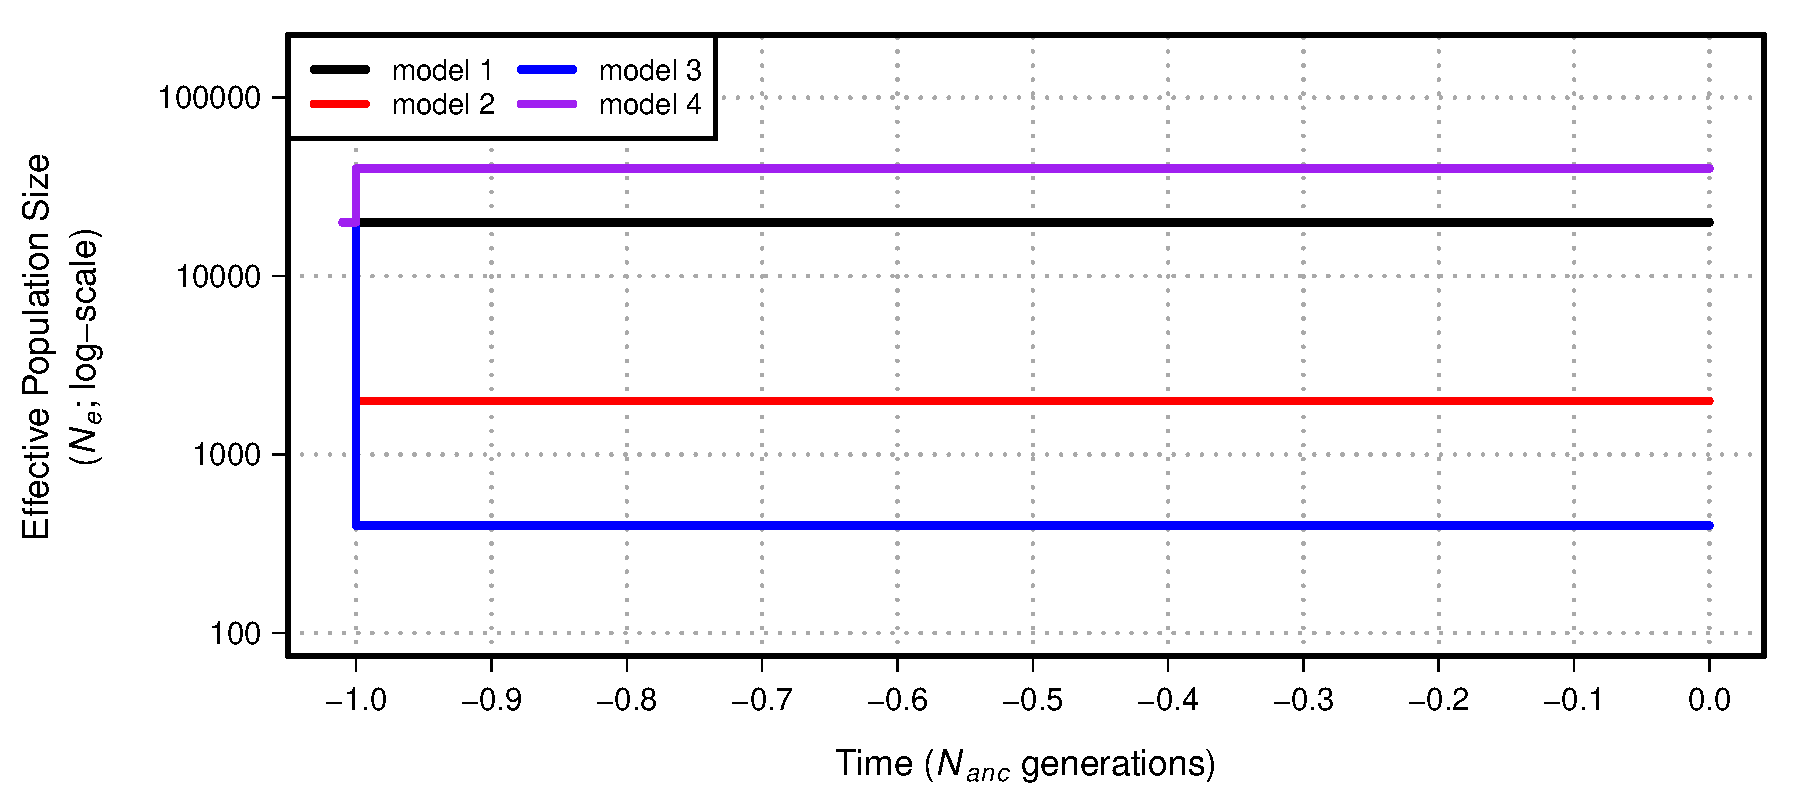
\includegraphics[width=0.8\linewidth]{figures/FigS1.pdf}
\caption{Demographic models 1-4 simulated in our study.
Time proceeds forward from left to right and is scaled by the $N_e$ of the population at the initial generation ($N_{anc}$; 20,000 individuals).
Demographic model 2 experiences a population contraction to 2000 individuals while demographic model 3 experiences a population contraction to 400 individuals.
Demographic model 4 experiences a population expansion to 40,000 individuals.
All population size changes are instantaneous for models 2-4.
See Table \ref{table:params} for additional model parameters.}
\label{fig:S1}
\end{figure*}
\pagebreak

\begin{figure*}[t]
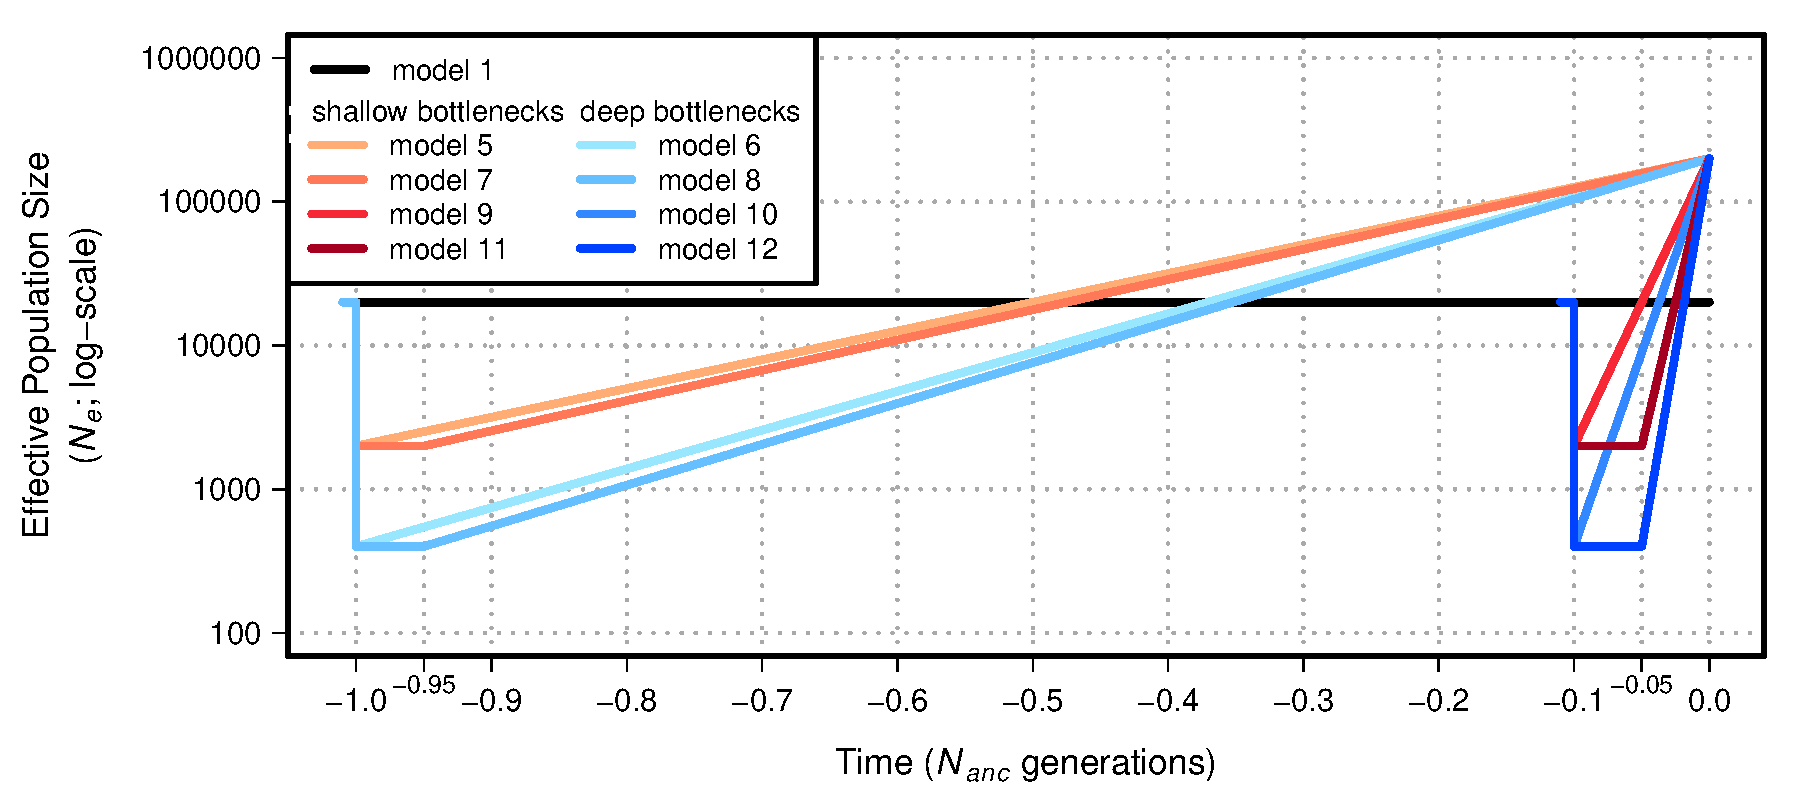
\includegraphics[width=0.8\linewidth]{figures/FigS2.pdf}
\caption{Demographic models 1 and 5-12 simulated in our study.
Time proceeds forward from left to right and is scaled by the $N_e$ of the population at the initial generation ($N_{anc}$; 20,000 individuals).
Demographic models with a shallow bottleneck (models 5, 7, 9, and 11) experience a population contraction to 2000 individuals while demographic models with a deep bottleneck (models 6, 8, 10, and 12) experience a population contraction to 400 individuals.
After contraction, demographic models 5-12 undergo exponential growth to a final population size of 200,000 individuals.
See Table \ref{table:params} for additional model parameters.}
\label{fig:S2}
\end{figure*}
\pagebreak

\begin{figure*}[t]
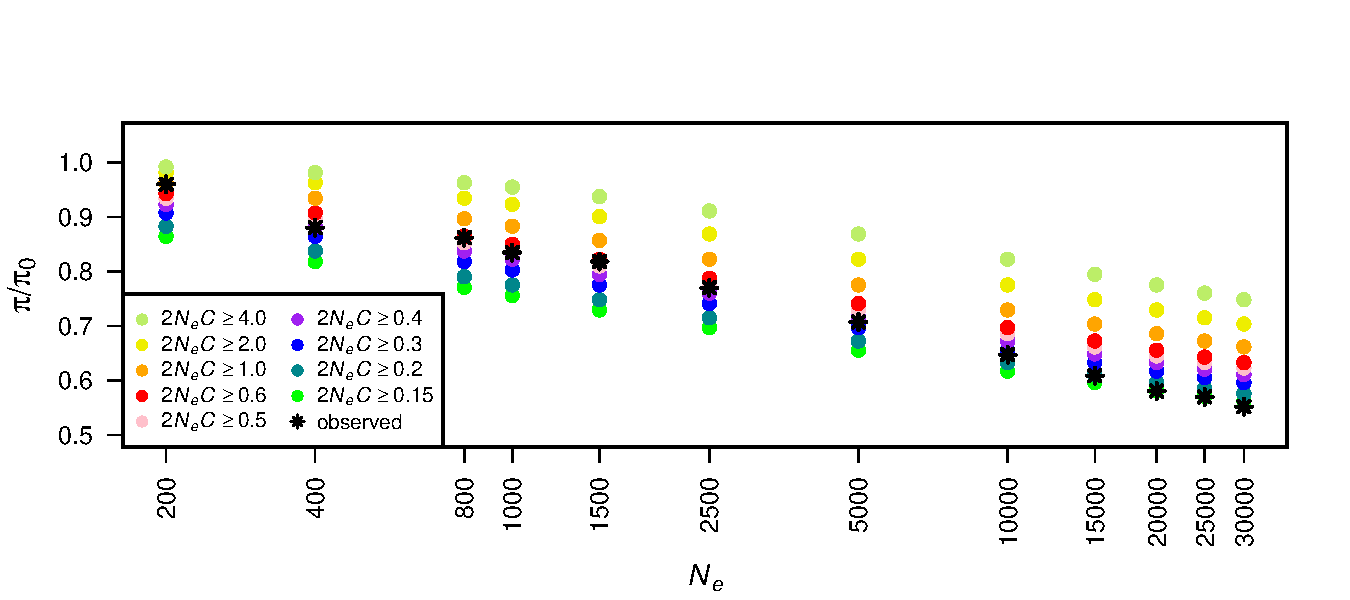
\includegraphics[width=.9\linewidth]{figures/FigS21.pdf}
\caption{Estimate of $\pi\pi_0$ from the Nordborg model across different population sizes and different truncation thresholds on selection.
Different $\gamma$ values used to truncate $s$ for the Nordborg model are shown in the legend ($2N_es \geq \gamma$).
Black stars represent the observed $\pi\pi_0$ from running simulations of BGS.}
\label{fig:nordborgsims}
\end{figure*}
\pagebreak

\begin{figure*}[t]
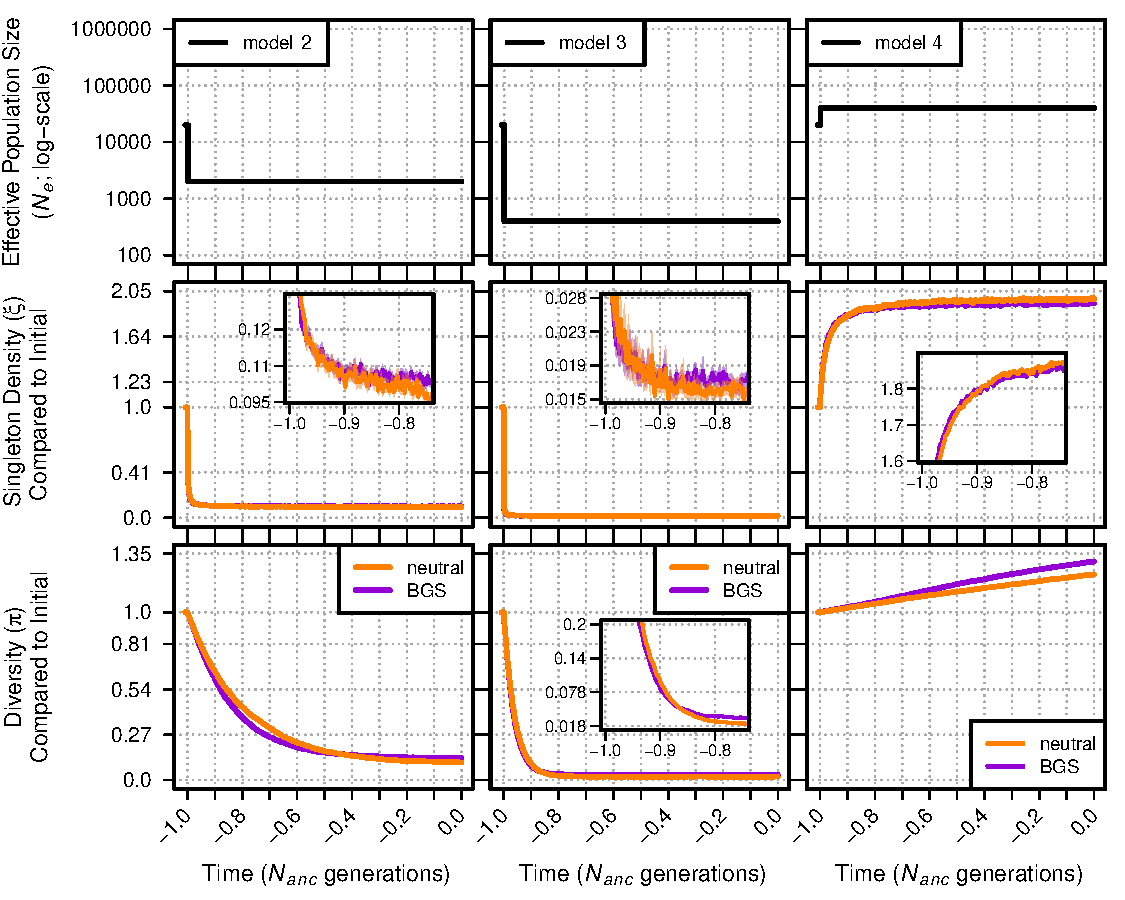
\includegraphics[width=.9\linewidth]{figures/FigS9.pdf}
\caption{Singleton density ($\xi$) and diversity ($\pi$) for demographic models 2-4 under neutrality (orange lines) and BGS (violet lines) relative to their values in the initial generation prior to demographic change.
The top panel shows each demographic model as in Figure \ref{fig:1}.
For greater detail, insets show data for generations over a smaller time scale and smaller y-axis (note: y-axes for insets are scaled linearly).
Envelopes are 95\% CIs calculated from 10,000 bootstraps of the original simulation data.
The data used for this figure is identical to that of Figure \ref{fig:1}.}
\label{fig:S9}
\end{figure*}
\pagebreak

\begin{figure}[t]
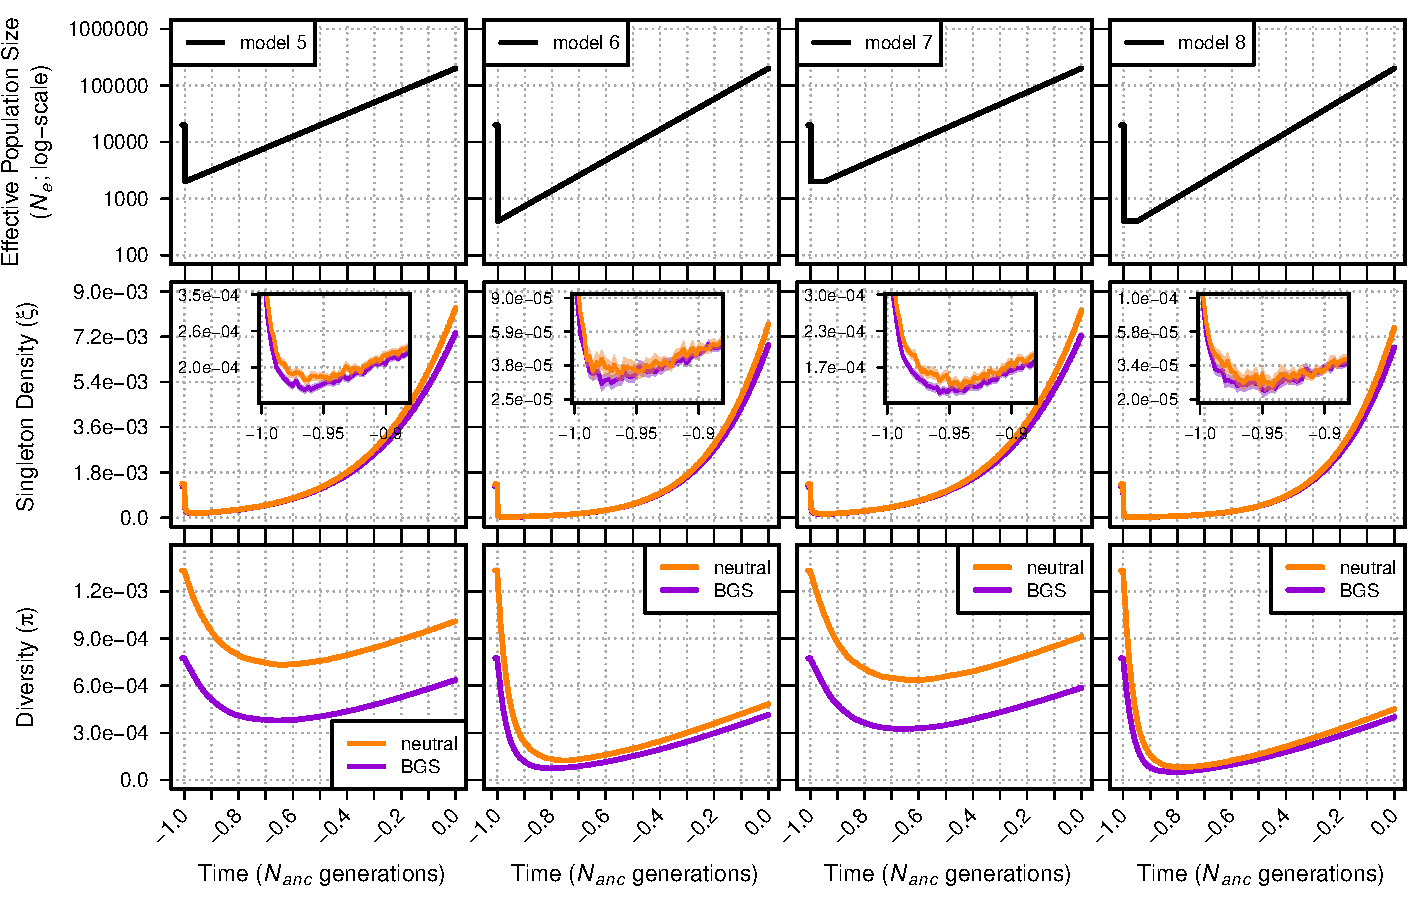
\includegraphics[width=\linewidth]{figures/FigS4.pdf}
\caption{Singleton density ($\xi$ per site) and diversity ($\pi$ per site) for models 5-8.
The top panel shows each demographic model; time proceeds forward from left to right and is scaled by the $N_e$ of the population at the initial generation ($N_{anc}$).
Diverstiy statistics are shown for neutral simulations (orange lines) and simulations with BGS (violet lines).
Insets show diversity using a log scale for improved detail.
Envelopes are 95\% CIs calculated from 10,000 bootstraps of the original simulation data.}
\label{fig:S4}
\end{figure}
\pagebreak

\begin{figure}[t]
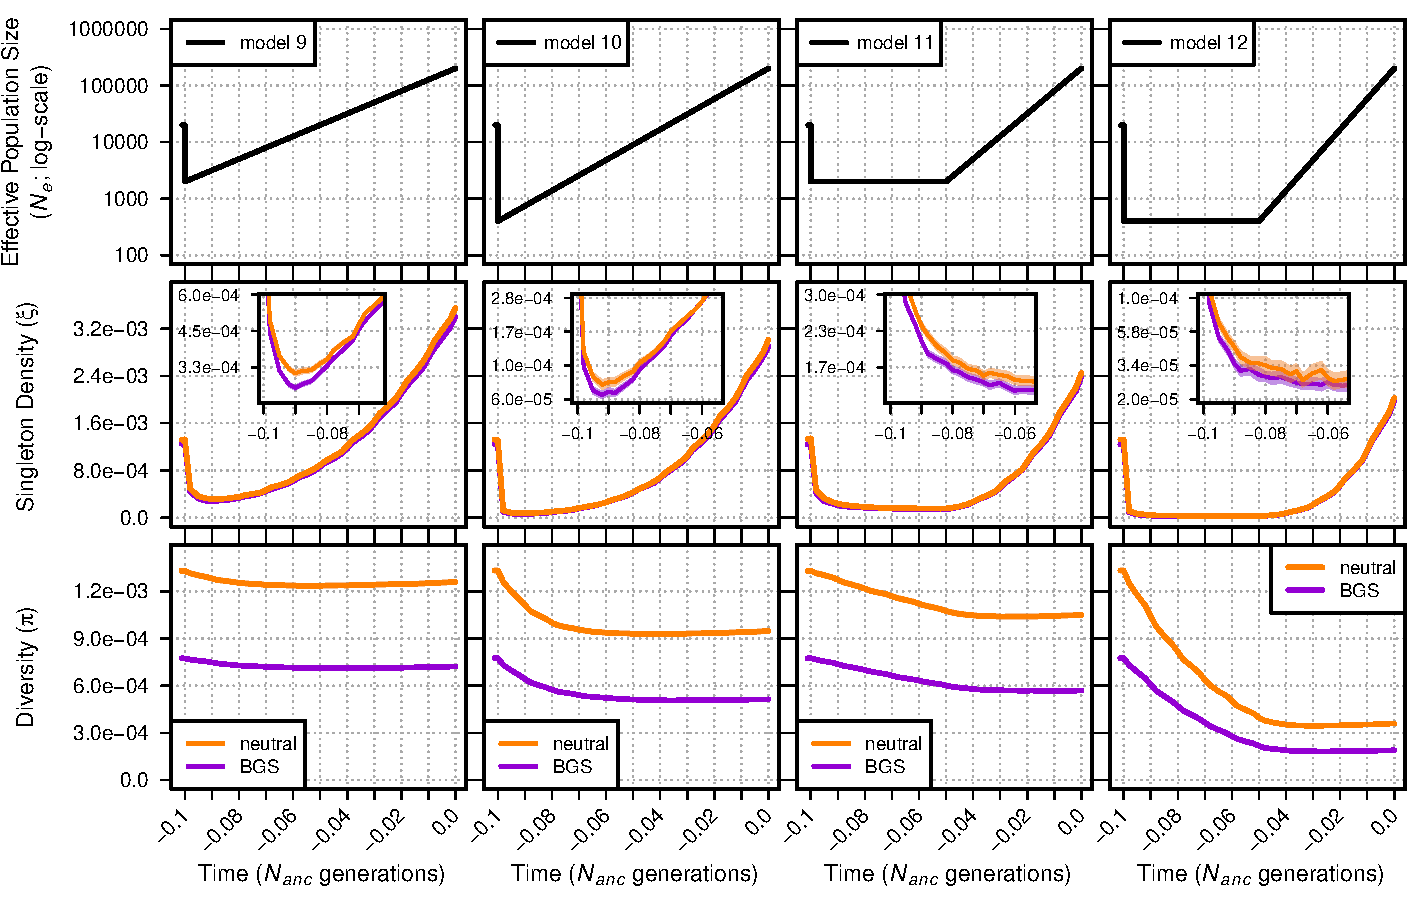
\includegraphics[width=\linewidth]{figures/FigS5.pdf}
\caption{Singleton density ($\xi$ per site) and diversity ($\pi$ per site) for models 9-12.
The top panel shows each demographic model; time proceeds forward from left to right and is scaled by the $N_e$ of the population at the initial generation ($N_{anc}$).
Diverstiy statistics are shown for neutral simulations (orange lines) and simulations with BGS (violet lines).
Insets show diversity using a log scale for improved detail.
Envelopes are 95\% CIs calculated from 10,000 bootstraps of the original simulation data.}
\label{fig:S5}
\end{figure}
\pagebreak

\begin{figure*}[h!]
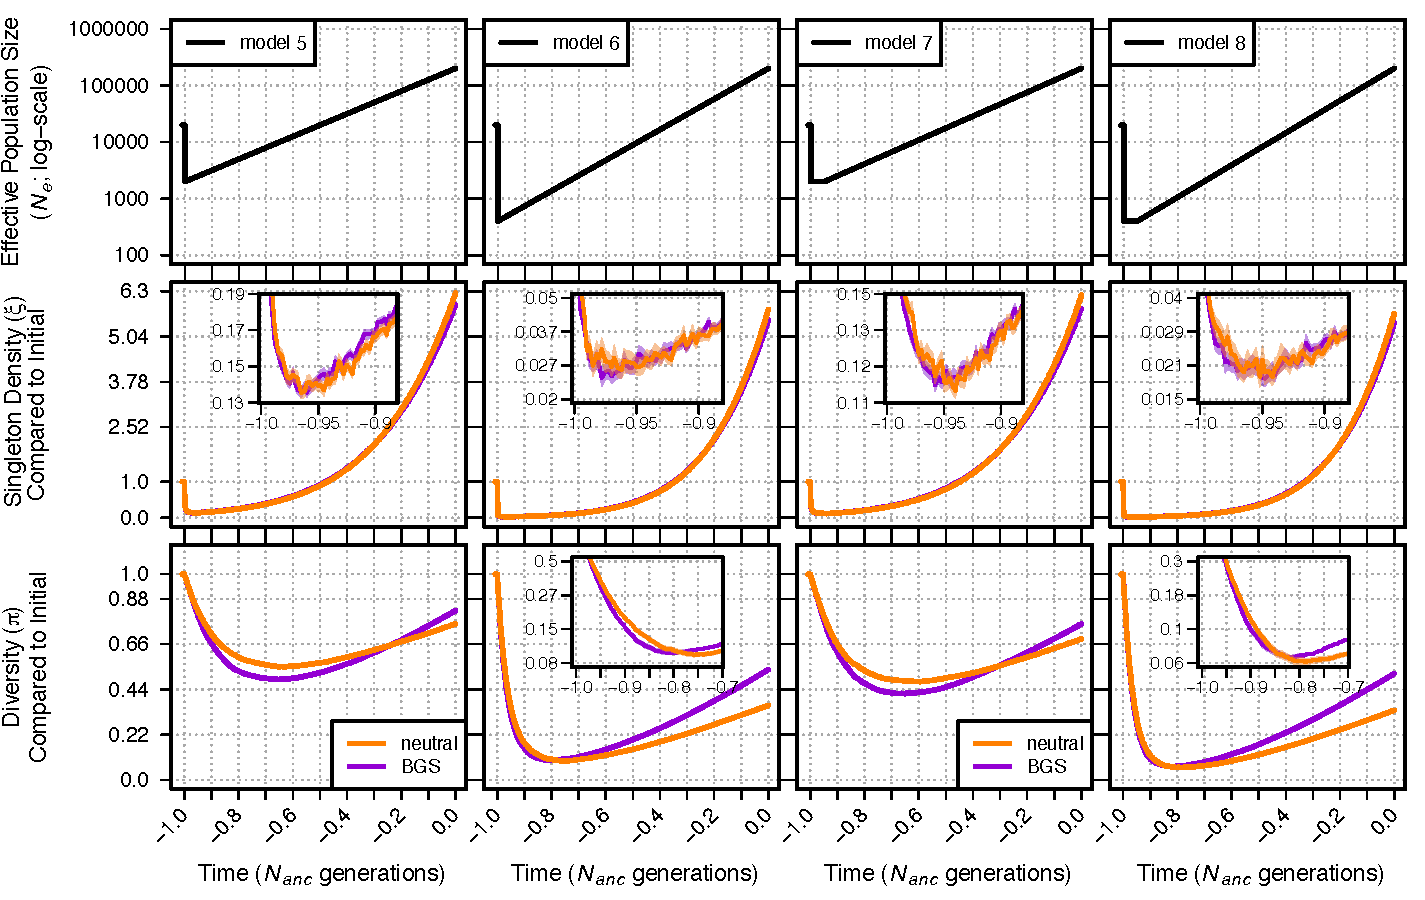
\includegraphics[width=0.8\linewidth]{figures/FigS7.pdf}
\caption{Singleton density ($\xi$ per site) and diversity ($\pi$ per site) relative to the initial generation for neutral (orange) and BGS (violet) simulations of demographic models 5-8.
The top panel shows each demographic model; time proceeds forward from left to right and is scaled by the $N_e$ of the population at the initial generation ($N_{anc}$).
Insets show diversity over a shorter timescale and use a log scale for diversity for improved detail.
Envelopes are 95\% CIs calculated from 10,000 bootstraps of the original simulation data.
The data used for this figure is identical to that of Supplemental Figure \ref{fig:S4}.}
\label{fig:S7}
\end{figure*}
\pagebreak

\begin{figure*}[h!]
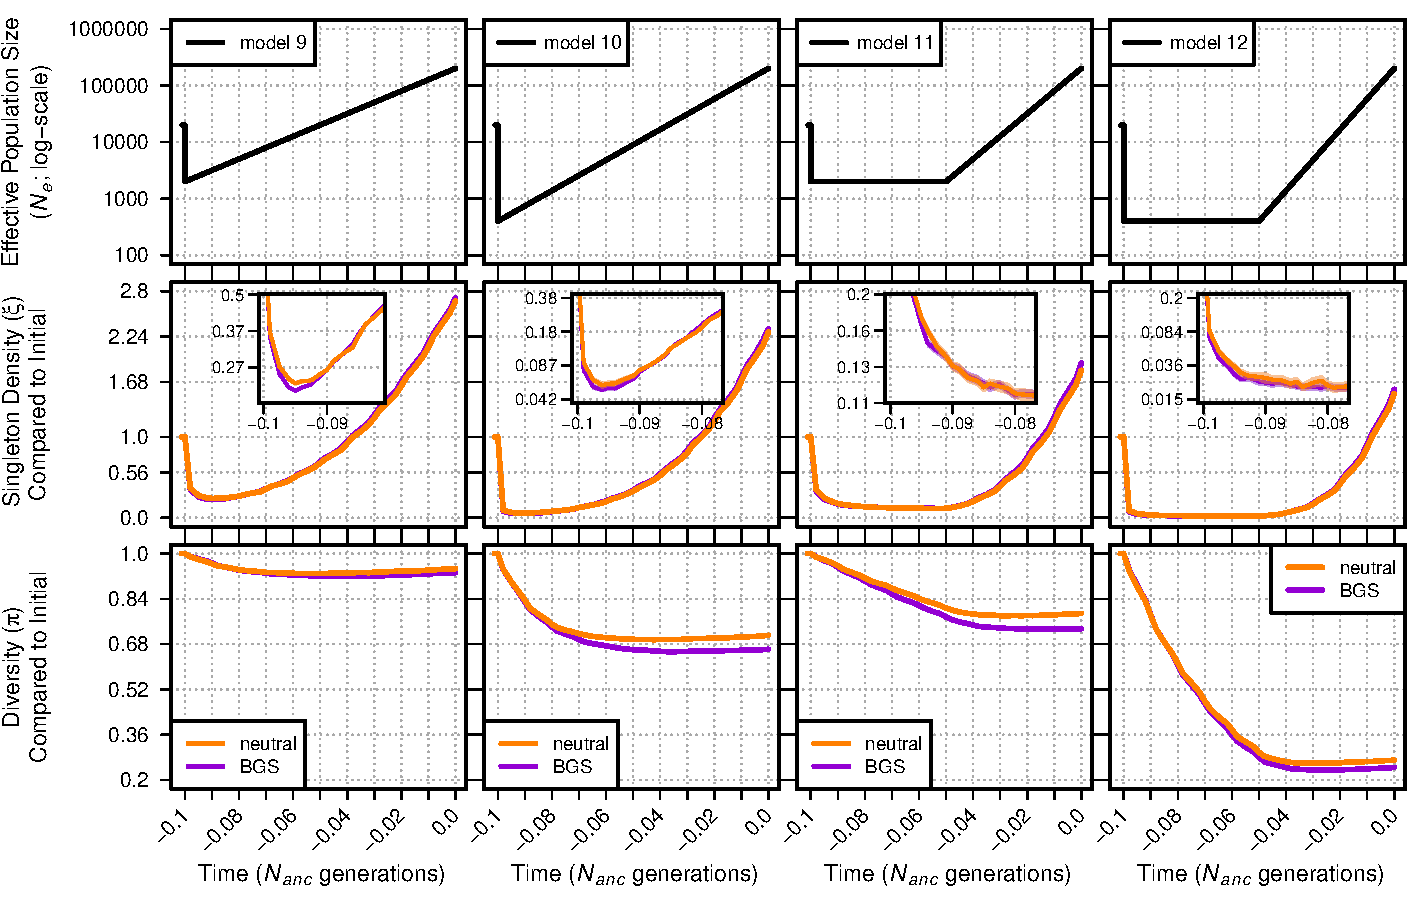
\includegraphics[width=0.8\linewidth]{figures/FigS8.pdf}
\caption{Singleton density ($\xi$ per site) and diversity ($\pi$ per site) relative to the initial generation for neutral (orange) and BGS (violet) simulations of demographic models 9-12.
The top panel shows each demographic model; time proceeds forward from left to right and is scaled by the $N_e$ of the population at the initial generation ($N_{anc}$).
Insets show diversity over a shorter timescale and use a log scale for diversity for improved detail.
Envelopes are 95\% CIs calculated from 10,000 bootstraps of the original simulation data.
The data used for this figure is identical to that of Supplemental Figure \ref{fig:S4}.}
\label{fig:S8}
\end{figure*}
\pagebreak

\begin{figure}[]
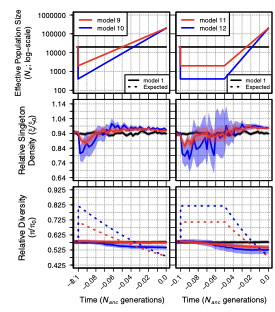
\includegraphics[width=0.5\linewidth]{figures/figsup912.png}
\caption{Relative singleton density ($\xi/\xi_0$) and relative diversity ($\pi/\pi_0$) across time for demographic models 1 and 9-12.
The top panel shows each demographic model as in Figure \ref{fig:1}.
Black lines show $\xi/\xi_0$ and $\pi/\pi_0$ from simulations of a constant sized population (model 1).
Dotted lines in the bottom panel show the equilibrium  expectation of $\pi/\pi_0$ from  \citet{nordborg1996effect} given the specific selection parameters and the instantaneous $N_e$ at each time point.
Envelopes are 95\% CIs calculated from 10,000 bootstraps of the original simulation data.}
\label{fig:S912}
\end{figure}
\pagebreak

\begin{figure}[htb]
    \centering
    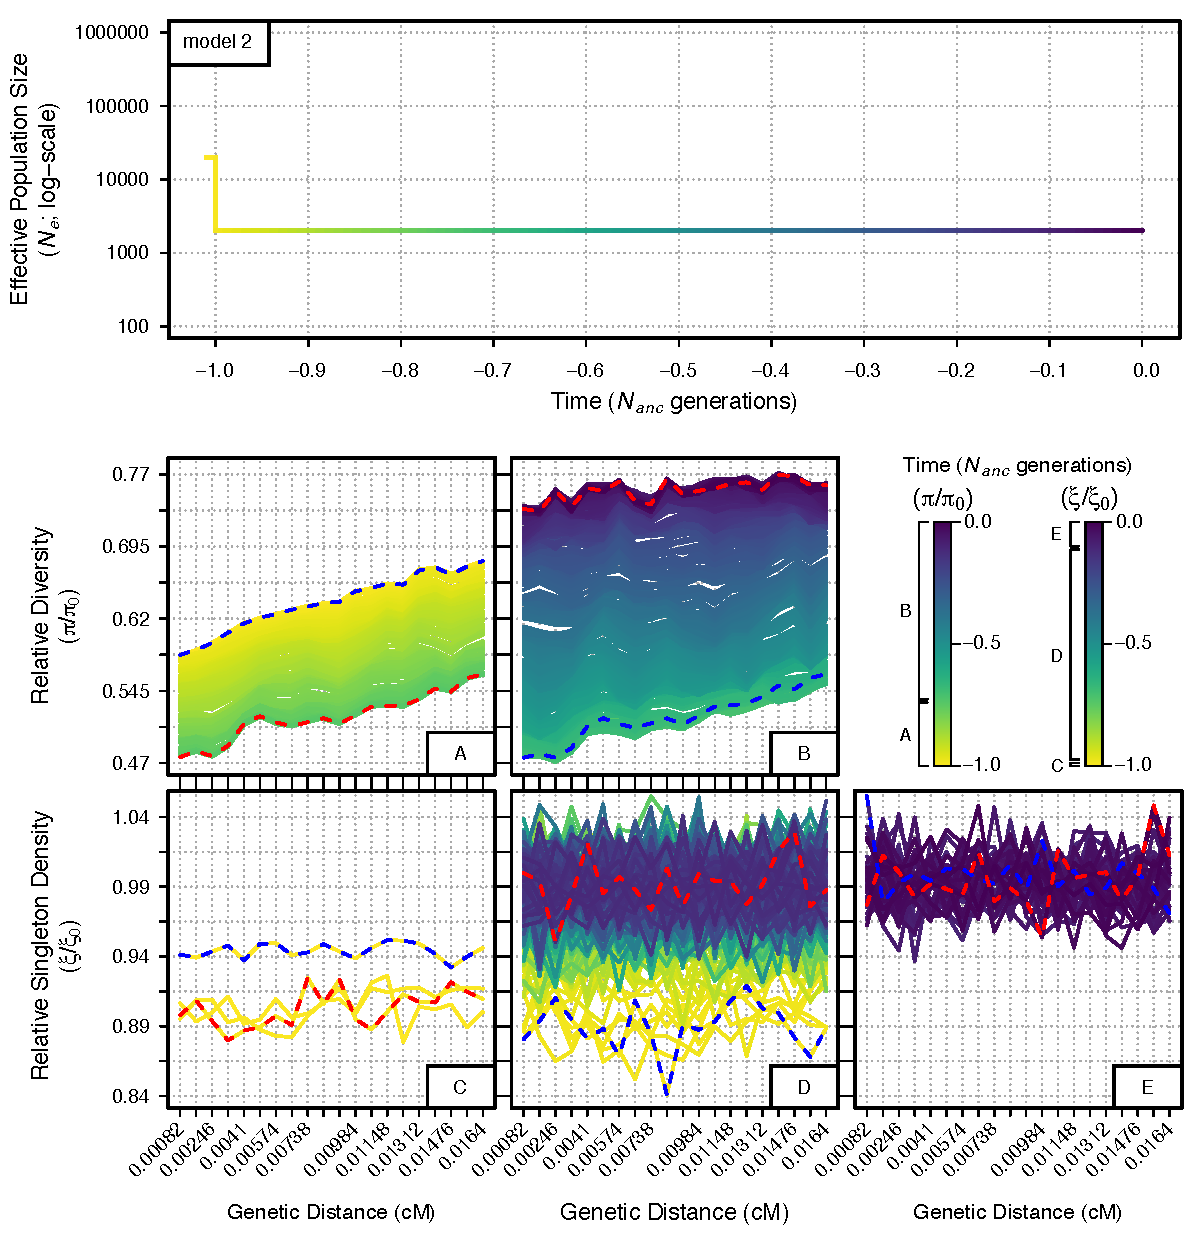
\includegraphics[width=\linewidth]{figures/FigS10.pdf}
\end{figure}
\begin{figure}[htb]\ContinuedFloat
    \centering
    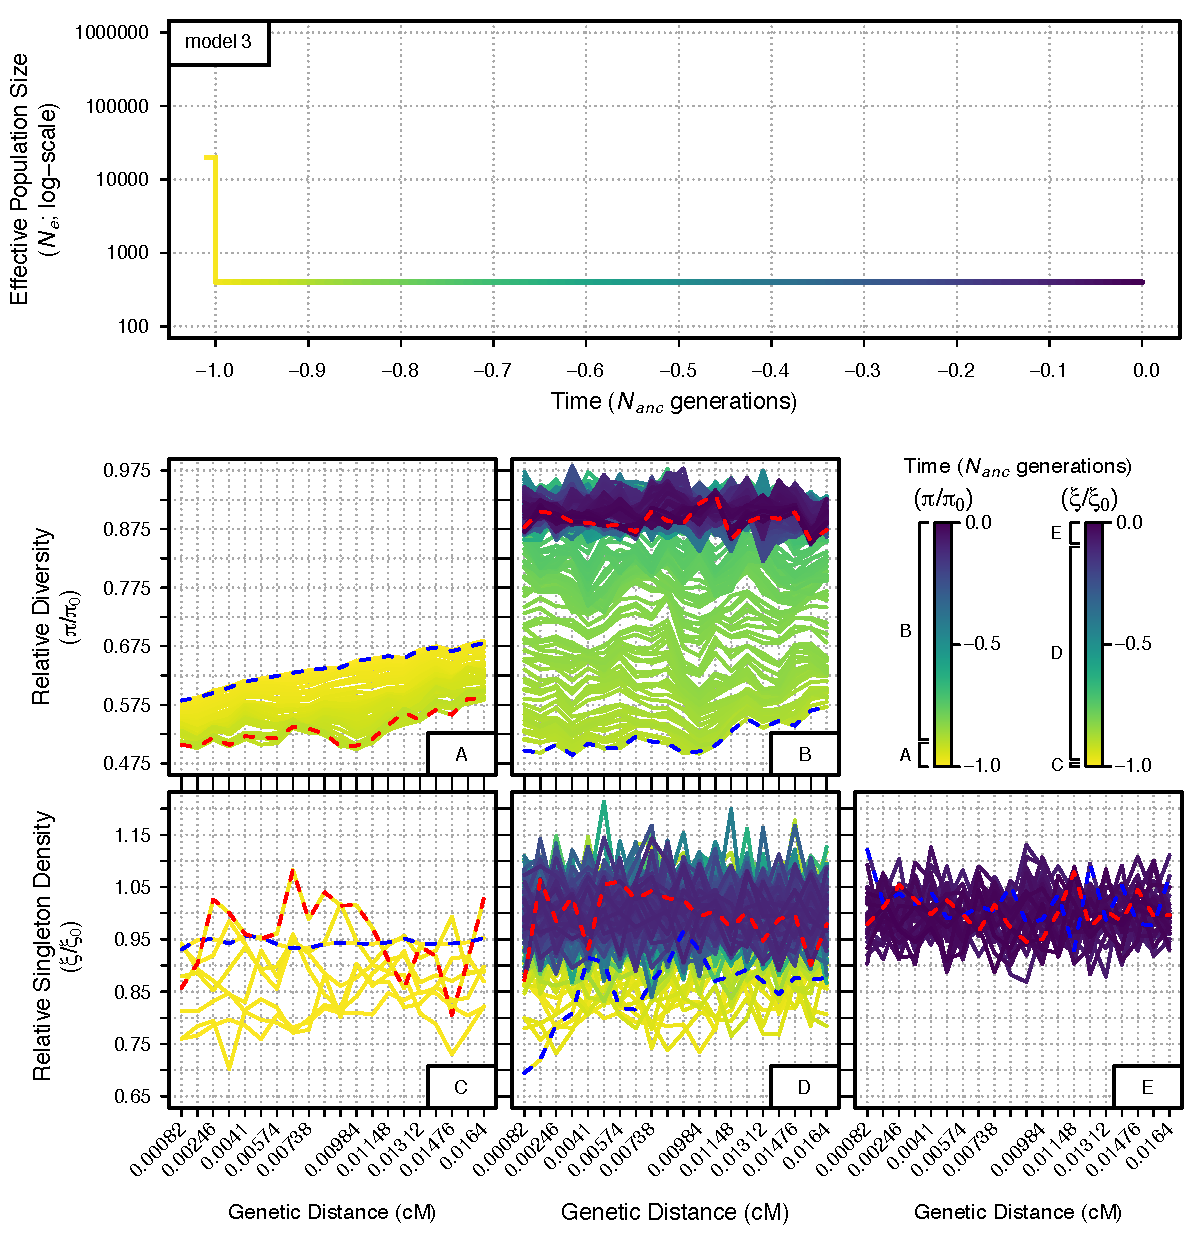
\includegraphics[width=\linewidth]{figures/FigS11.pdf}
\end{figure}
\begin{figure}[htb]\ContinuedFloat
    \centering
    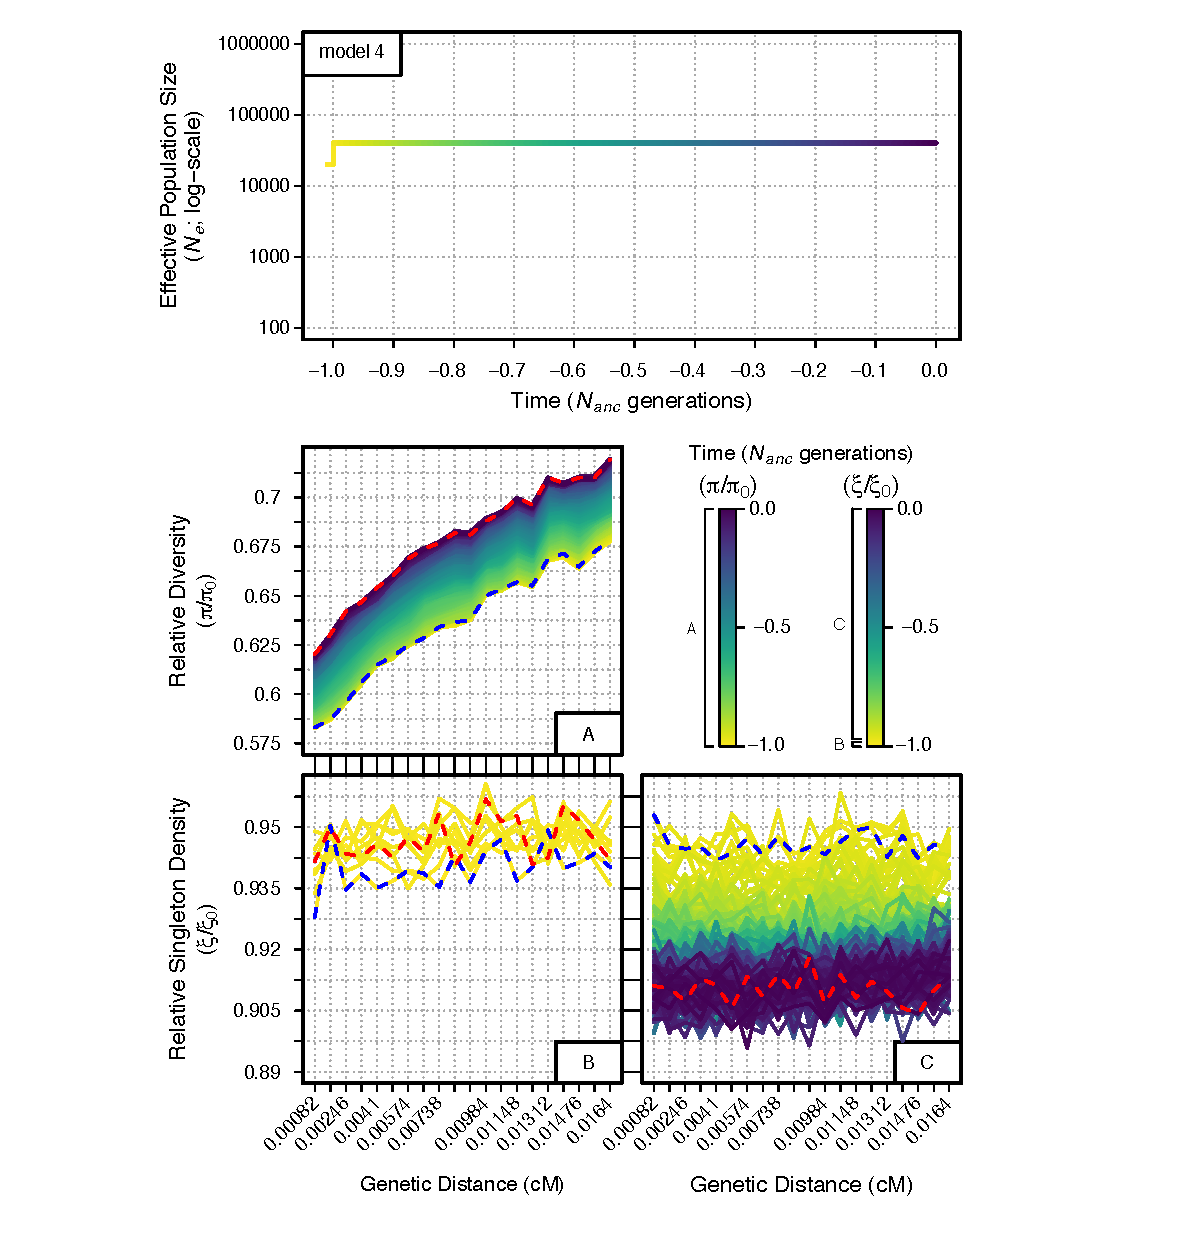
\includegraphics[width=\linewidth]{figures/FigS12.pdf}
\end{figure}
\begin{figure}[htb]\ContinuedFloat
    \centering
    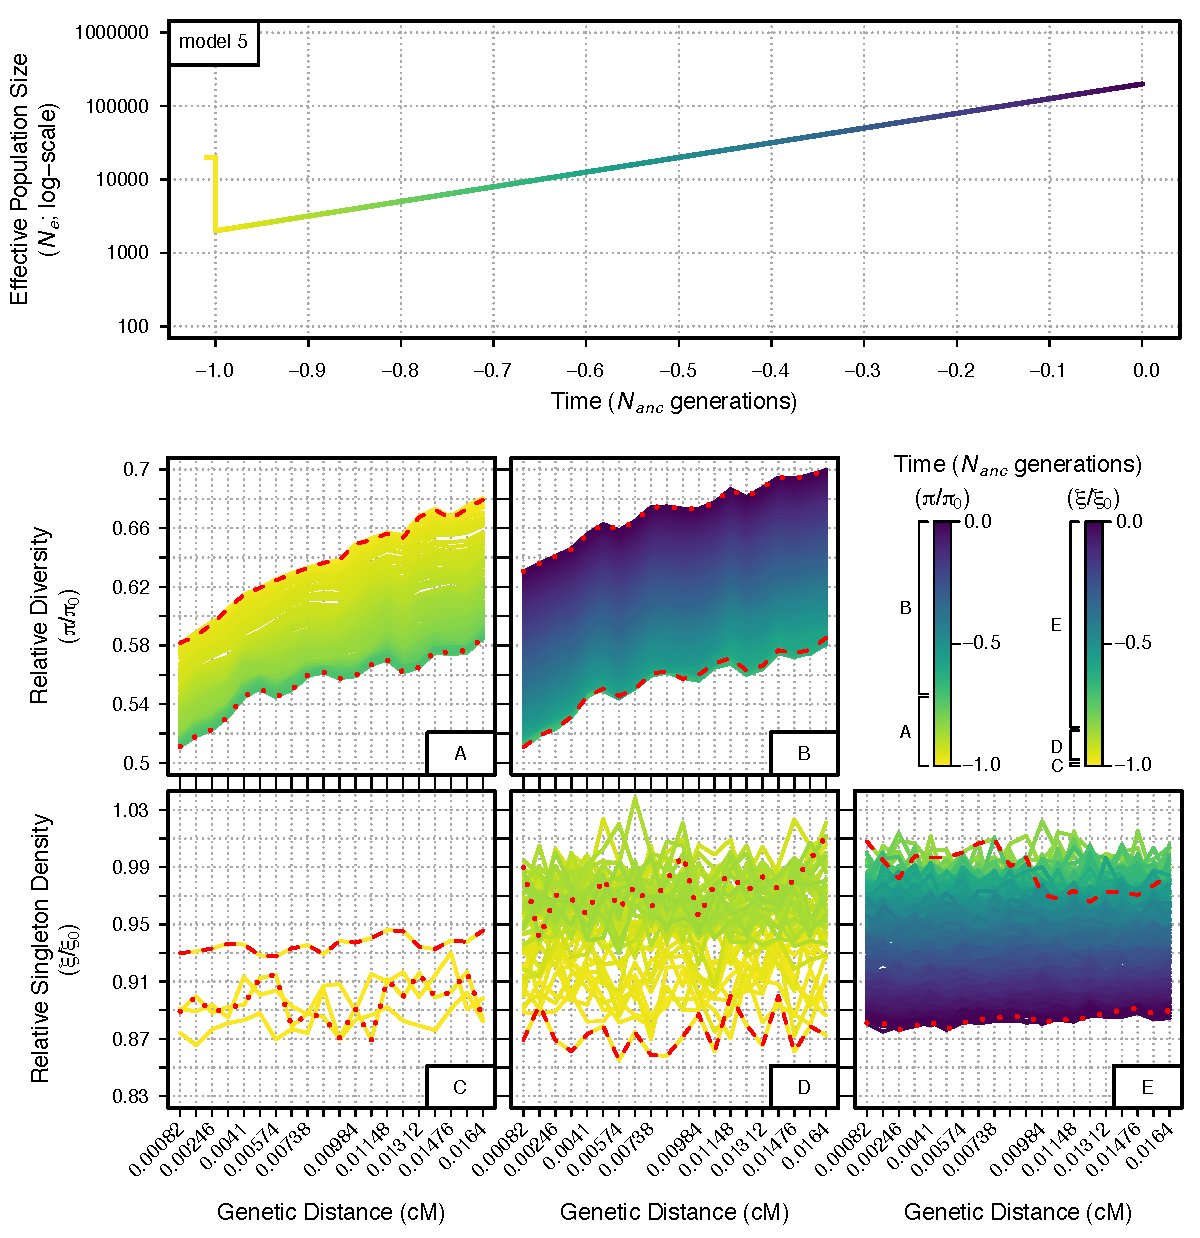
\includegraphics[width=\linewidth]{figures/FigS13.pdf}
\end{figure}
\begin{figure}[htb]\ContinuedFloat
    \centering
    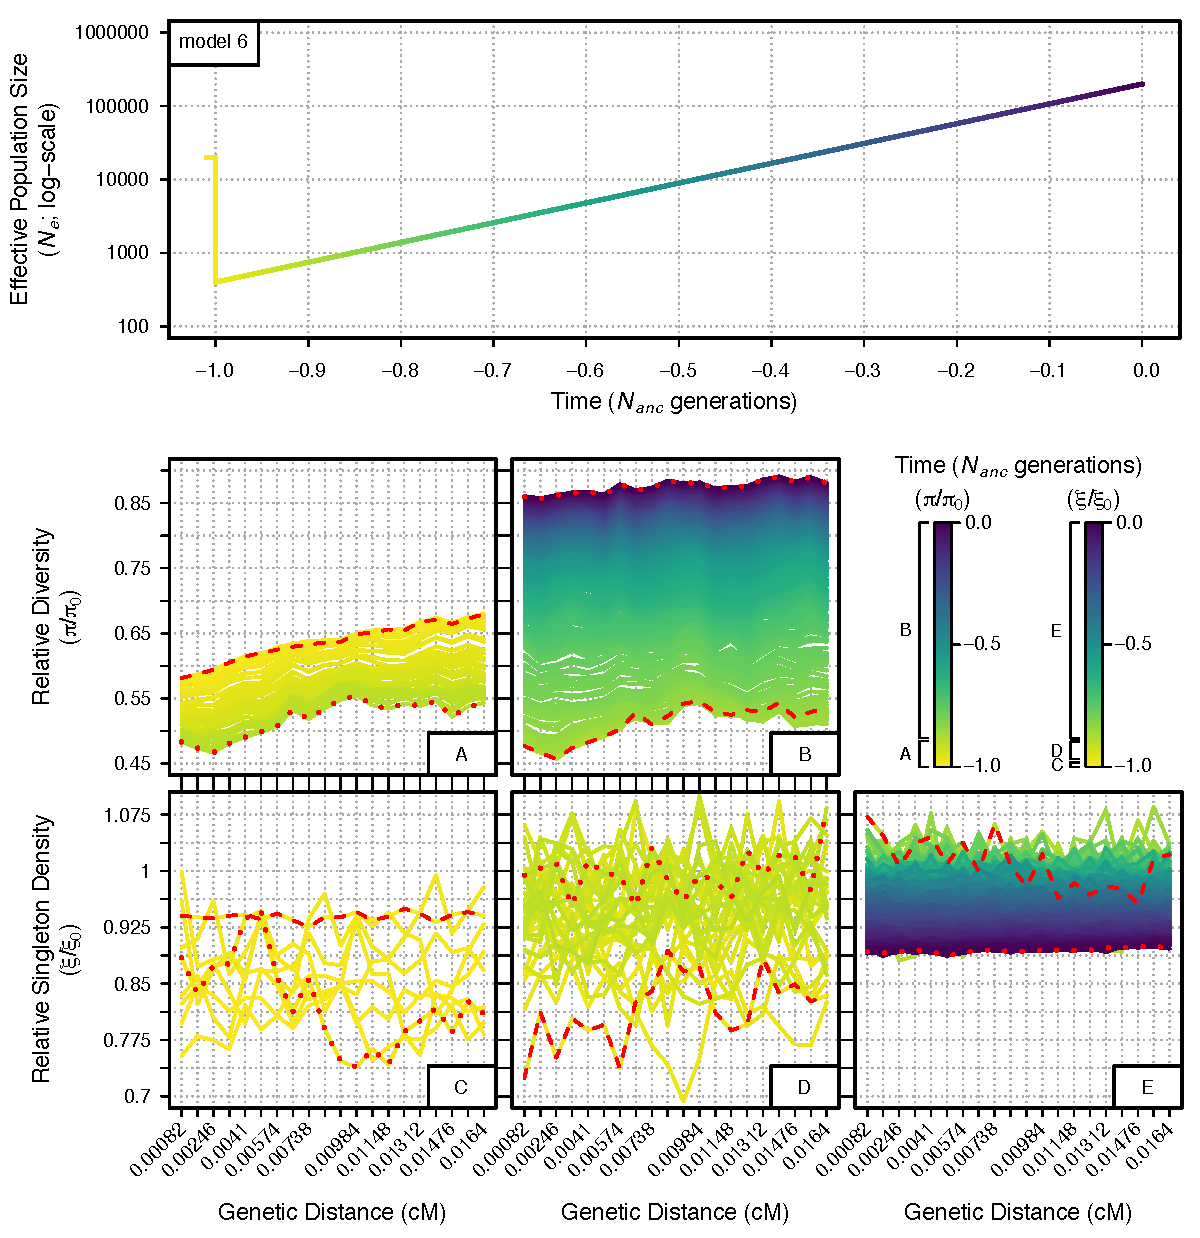
\includegraphics[width=\linewidth]{figures/FigS14.pdf}
\end{figure}
\begin{figure}[htb]\ContinuedFloat
    \centering
    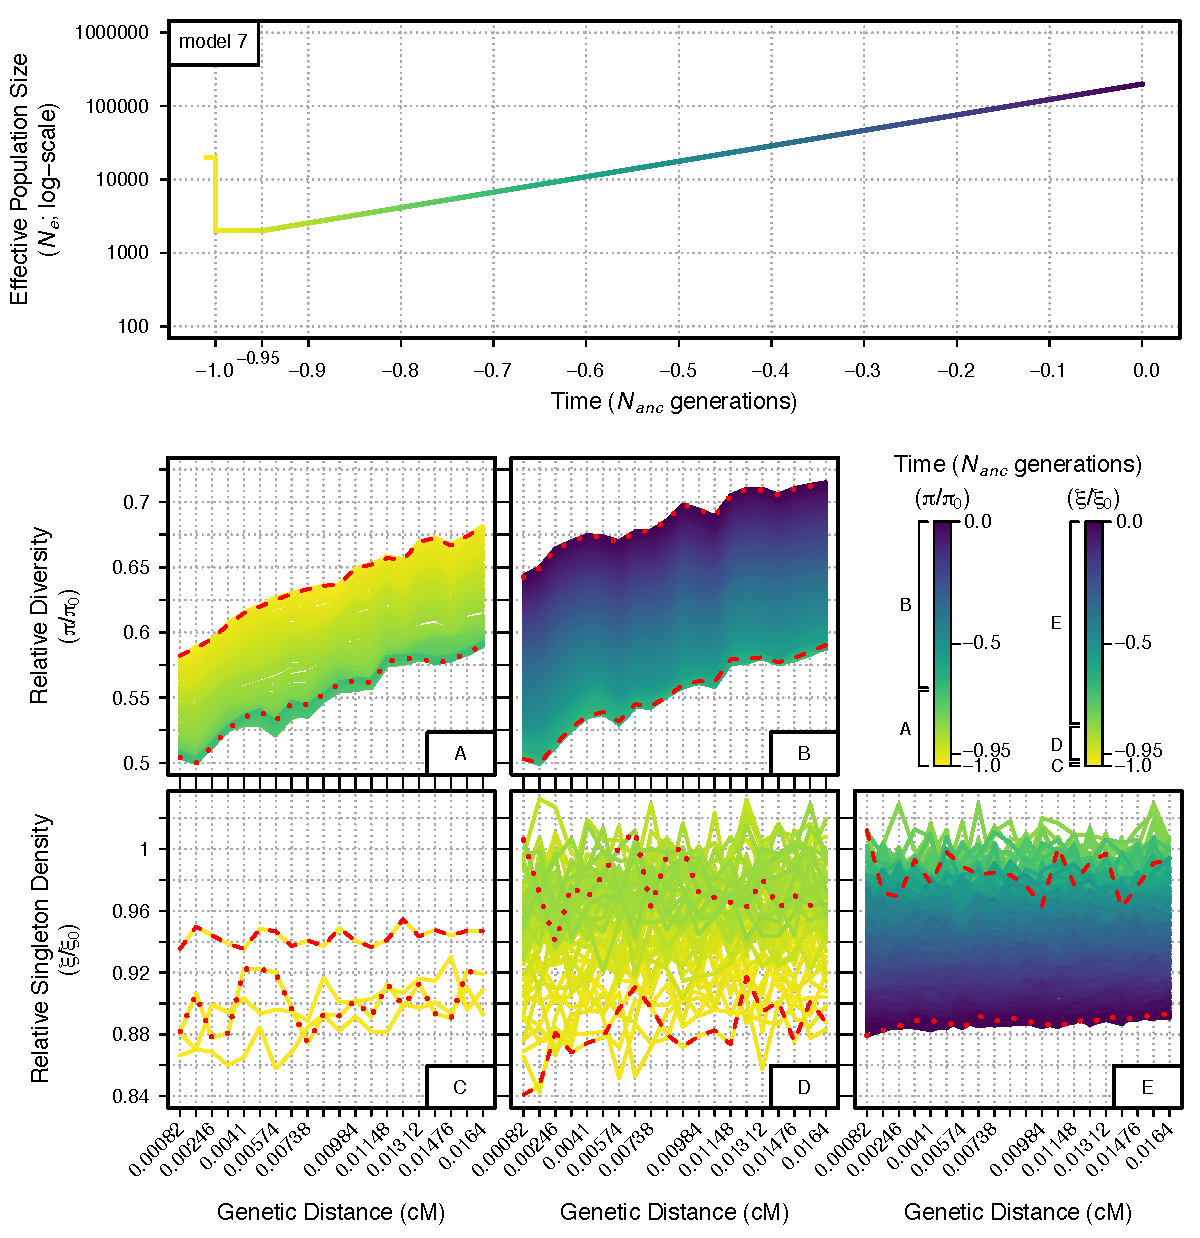
\includegraphics[width=\linewidth]{figures/FigS15.pdf}
\end{figure}
\begin{figure}[htb]\ContinuedFloat
    \centering
    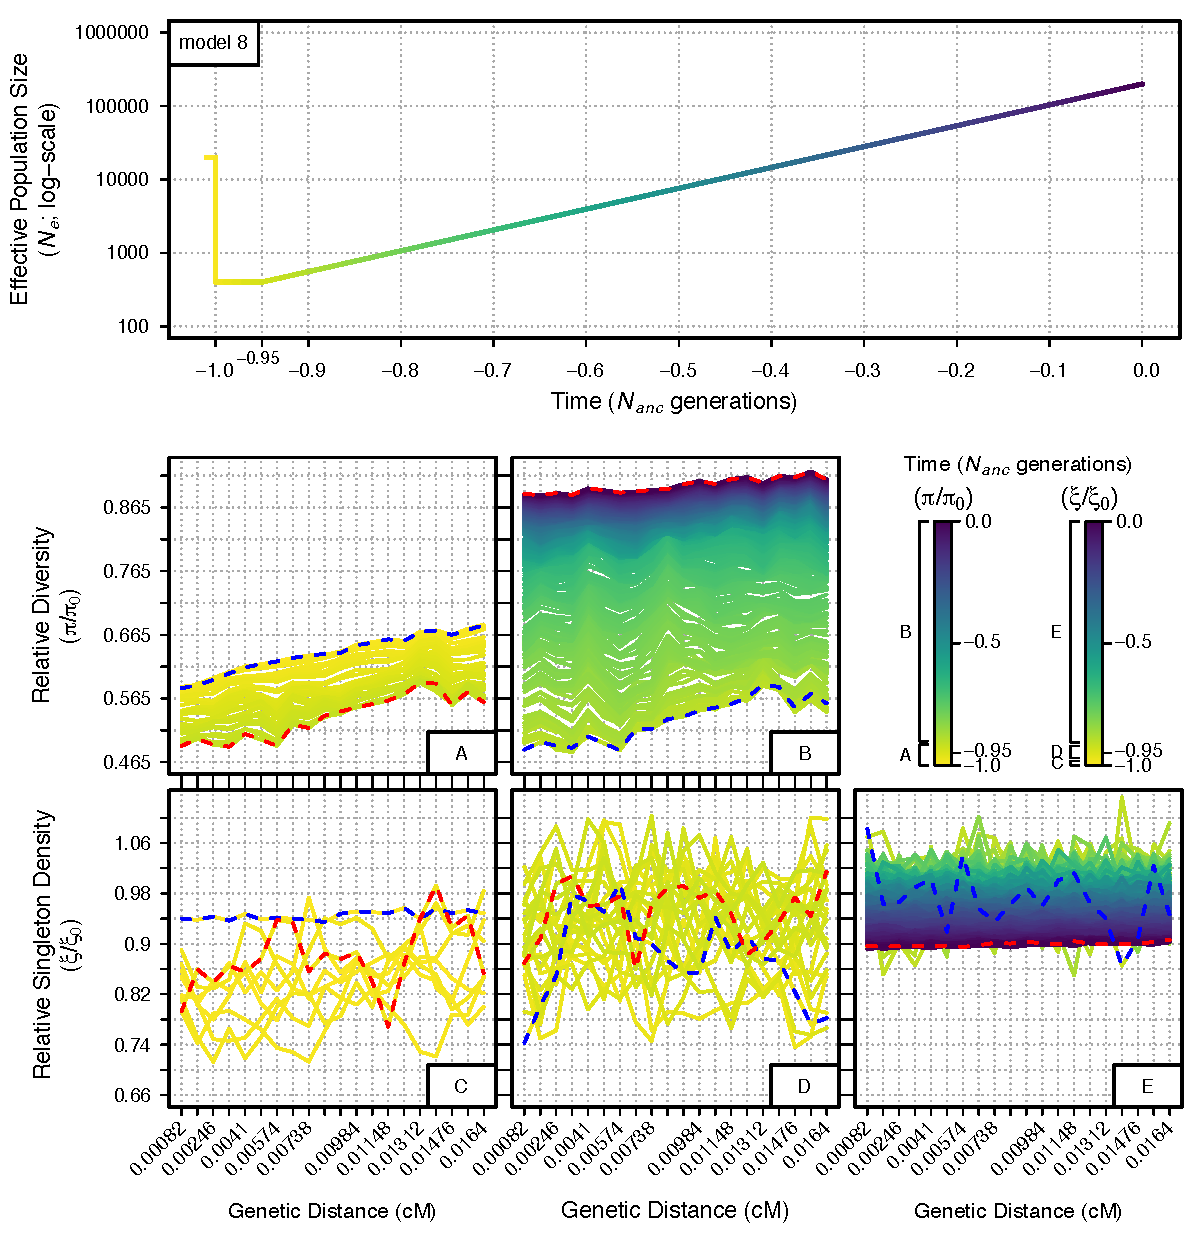
\includegraphics[width=\linewidth]{figures/FigS16.pdf}
\end{figure}
\begin{figure}[htb]\ContinuedFloat
    \centering                   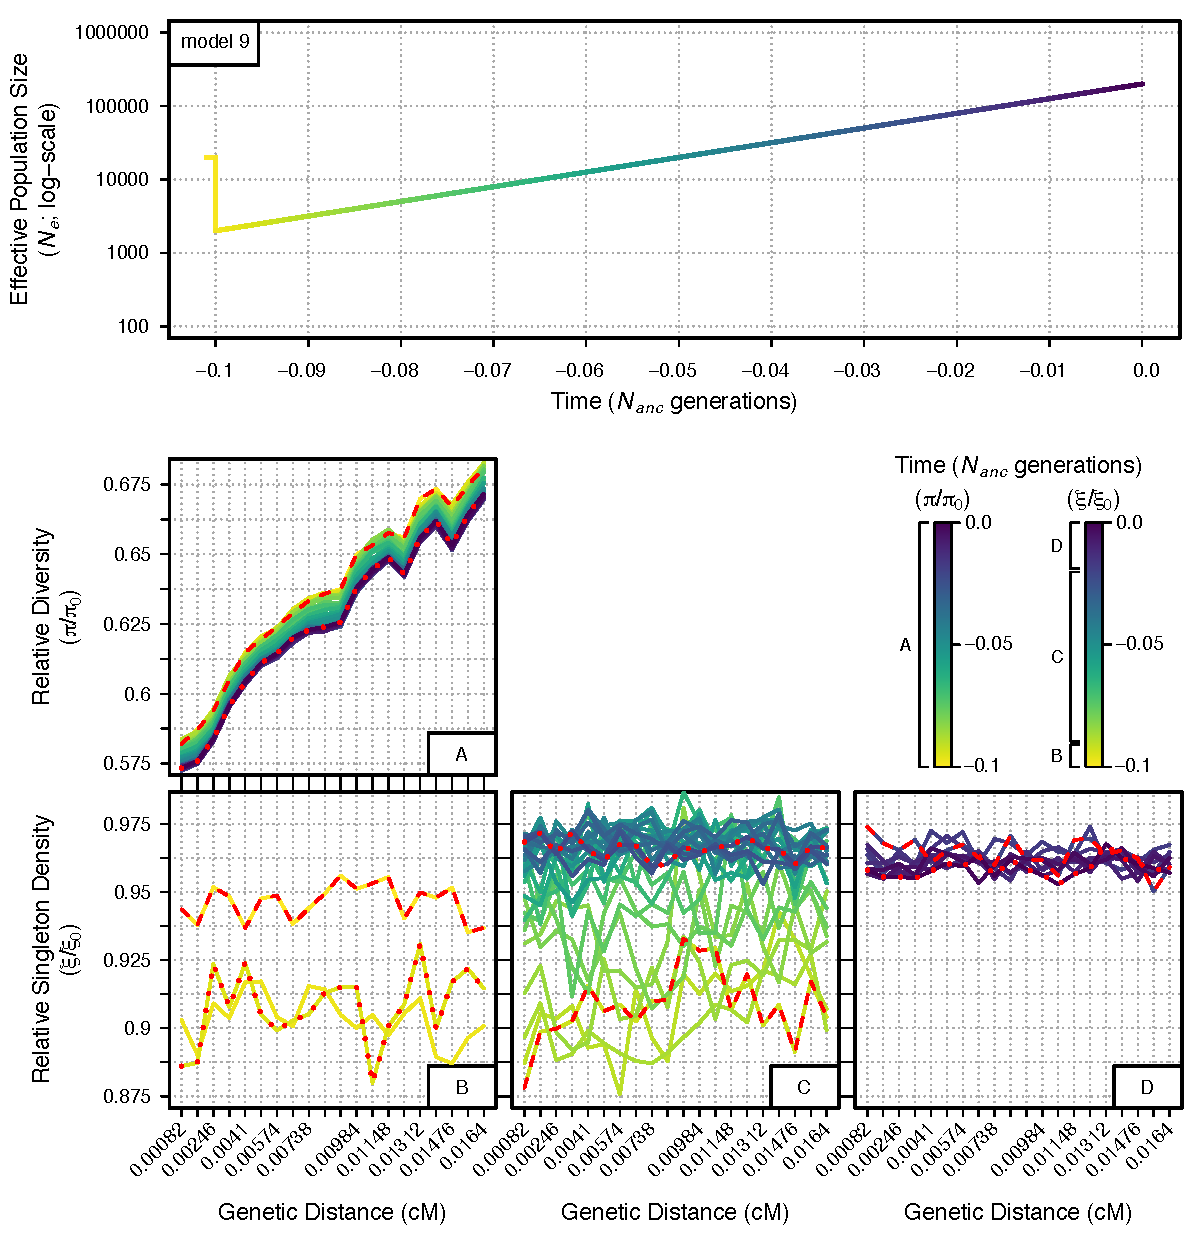
\includegraphics[width=\linewidth]{figures/FigS17.pdf}
\end{figure}
\begin{figure}[htb]\ContinuedFloat
      \centering
      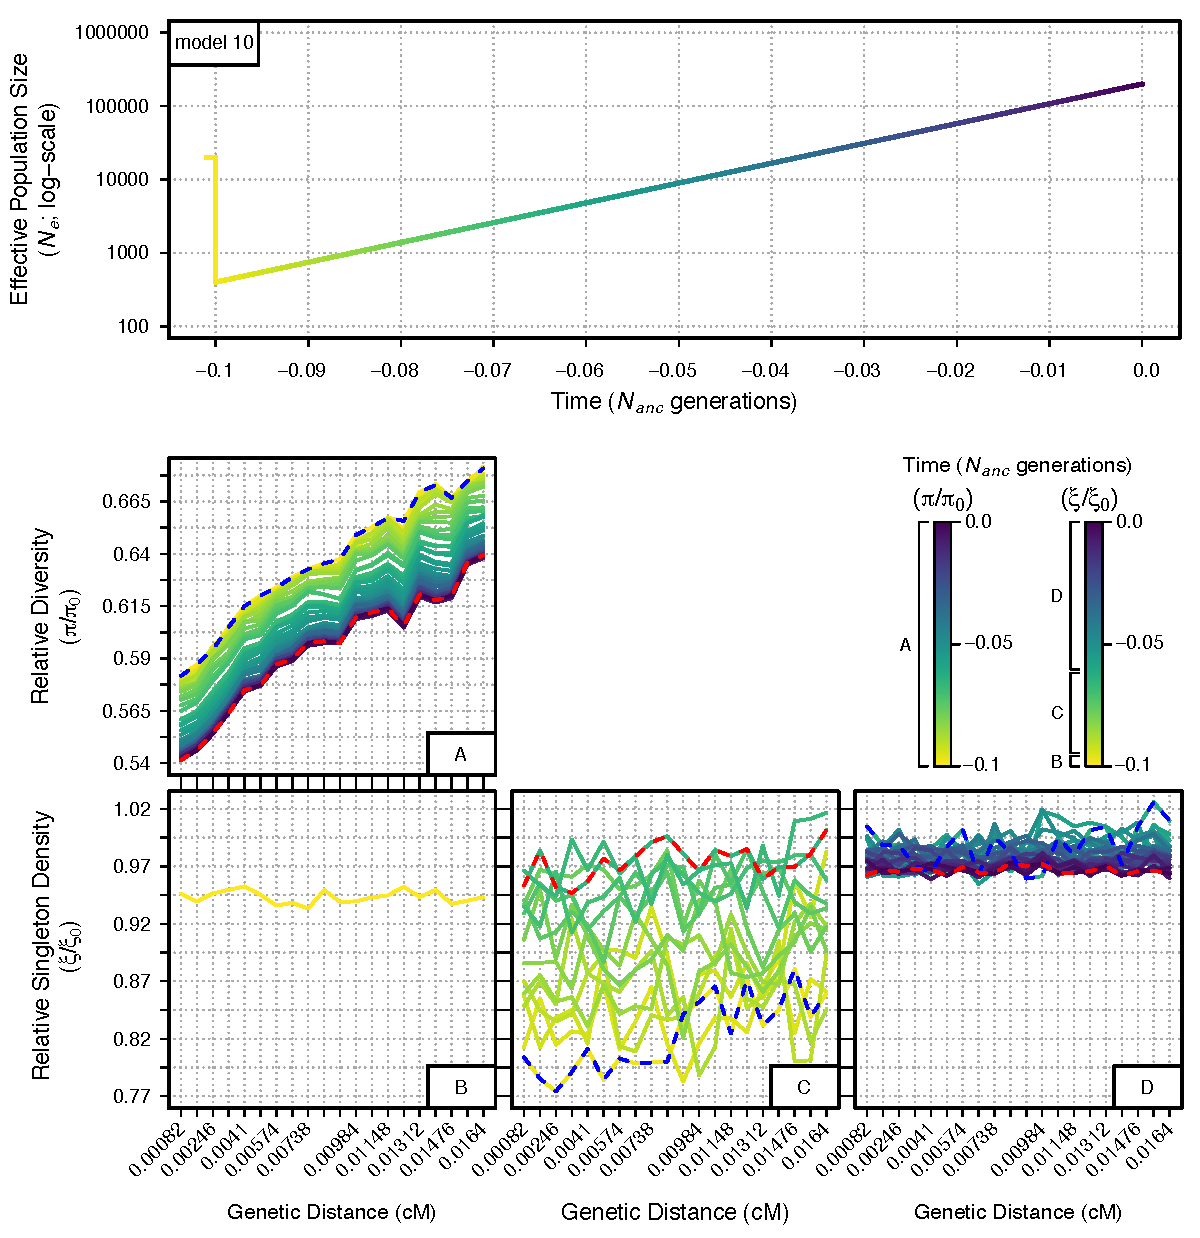
\includegraphics[width=\linewidth]{figures/FigS18.pdf}
\end{figure}
\begin{figure}[htb]\ContinuedFloat
      \centering
      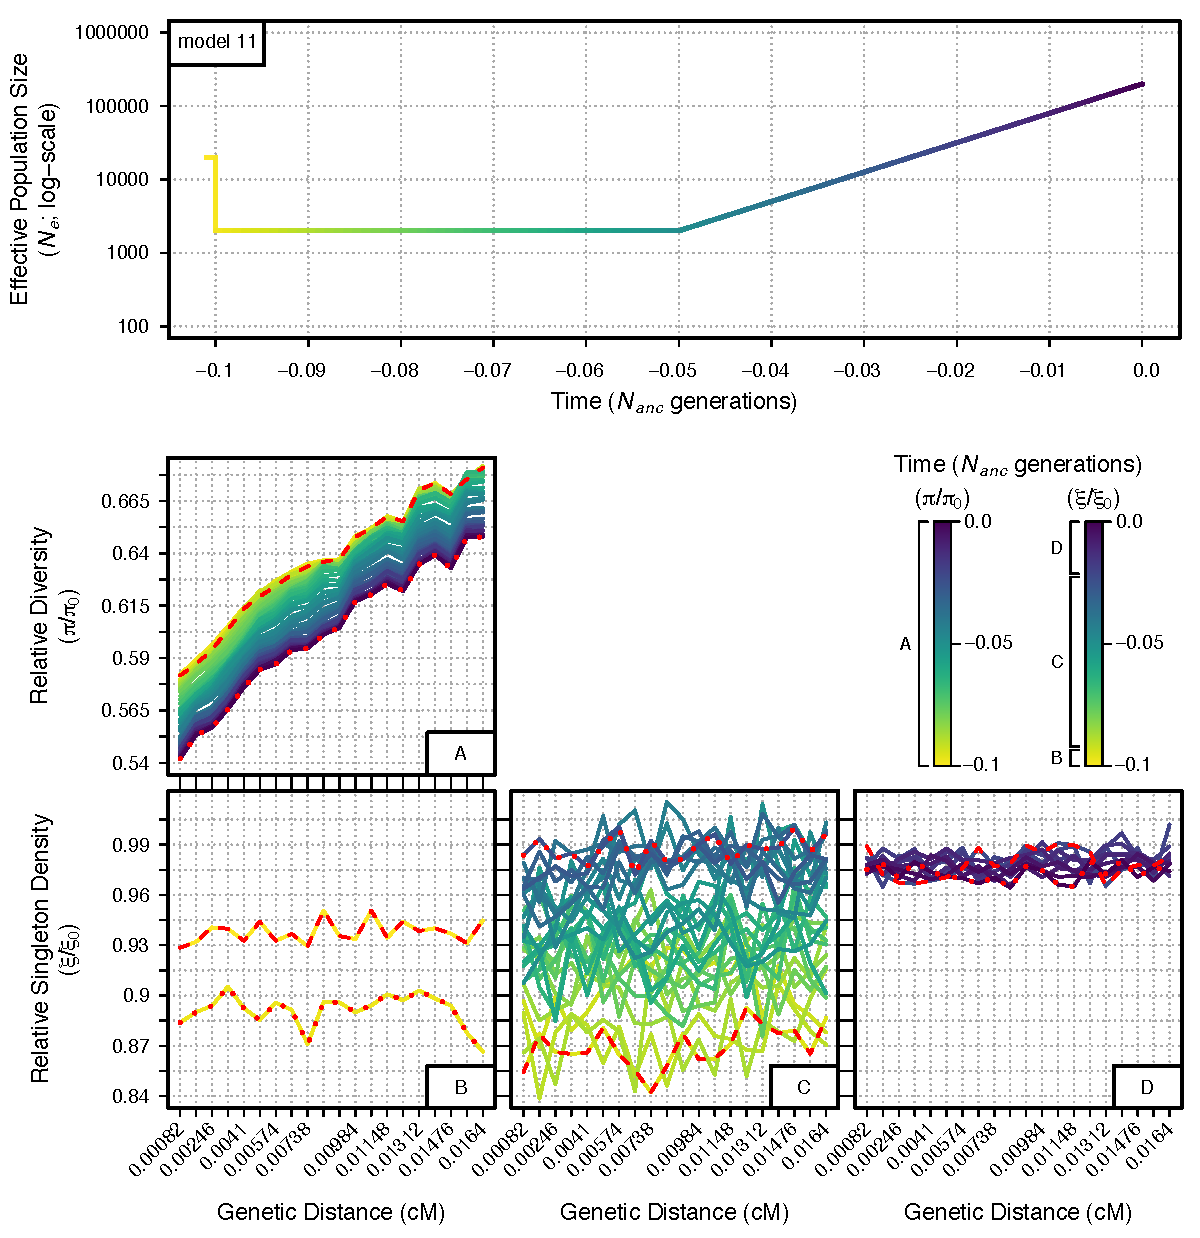
\includegraphics[width=\linewidth]{figures/FigS19.pdf}
\end{figure}
\begin{figure}[htb]
      \centering
      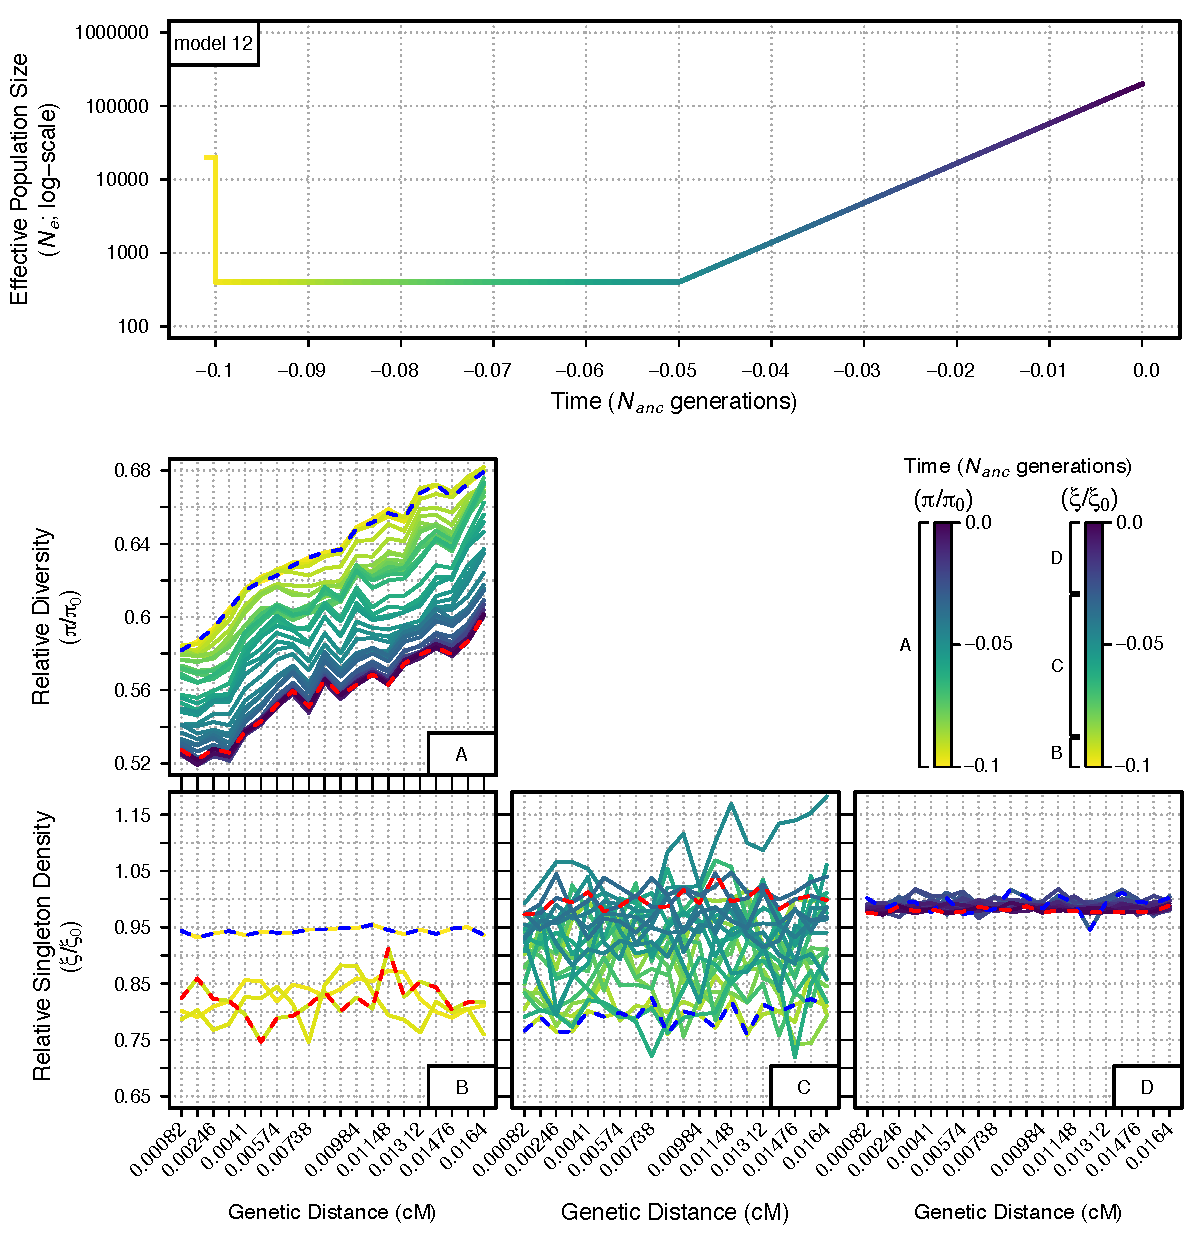
\includegraphics[width=\linewidth]{figures/FigS20.pdf}
      \caption{Relative diversity ($\pi/\pi_0$) and singleton density ($\xi/\xi_0$) through time for demographic models 2-12 measured across a neutral 200 kb region under the effects of BGS.
The genetic distance of each 10 kb bin from the selected locus is indicated on the x-axes, with genetic distance increasing from left to right.
Each line measuring $\pi/\pi_0$ and $\xi/\xi_0$ across the 200 kb neutral region represents a specific generation of the demographic model (401 discrete generations for demographic models 2-8, 41 discrete generations for demographic models 9-12).
Specific generations are indicated by the color of the demographic model at the top of each figure (time is scaled as in Figure \ref{fig:s6}) and in the figure legend.
When necessary, multiple plots are given fori $\pi/\pi_0$ and $\xi/\xi_0$ in order to prevent overlap of the measurements between generations (see legend for specific generations covered in each plot).
Blue dashed lines and red dashed lines indicate the first generation and last generation measured, respectively, for each specific plot.}
\label{fig:S912}
\end{figure}
\pagebreak

% \begin{table*}[htbp]
% \centering

% \caption{\bf Shrink a large table to fit the page}
% %\begin{adjustbox}{totalheight=\textheight-2\baselineskip}
% \begin{tableminipage}{\textwidth}
% \begin{small}
% \begin{tabularx}{\textwidth}{sb}
% \hline
% Parameter & Description \\
% \hline
% \textbf{Adaptation} & \textbf{Trait related parameters} \\
% \hline
% Time to optimum & Generations until new optimum is reached \\
% Adaptation rate (haldane) & Adaptation rate until new optimum is reached. Calculated as $rate(h) = \frac{\frac{ln(x_2)}{sd_{x_{12}}}-\frac{ln(x_1)}{sd_{x_{12}}}}{t_2-t_1}$ \\
% Final genetic variance & Genetic variance in the final generation \\
% \textbf{Fixations} & \textbf{Mutations that fix after the optimum shift} \\
% \hline
% From new mutations (\#) & Sum of fixed mutations in the final population that were already segregating before  the optimum shift \\
% From standing variation (\#) & Sum of fixed mutations in the final population that arose after the optimum shift \\
% Max. effect size & Maximal effect size of all fixations \\
% Mean effect size & Mean effect size of all fixations \\
% Mean effect size of negative fixations & Mean effect size of negative mutations \\
% Mean effect size of positive fixations & Mean effect size of positive mutations \\
% Mean emergence time & Mean generation when a mutation arose that fixed in the last 0.1 N generations \\
% Mean fixation time & Mean generation in which a mutation fixed \\
% Min. effect size & Minimal effect size of all fixations \\
% Negative (\#) & Sum of fixed mutations with negative effects in the final population \\
% New/standing fixations & Ratio of mutations from new mutations vs. standing mutations  \\
% Proportion negative & Proportion of negative fixations from all mutations \\
% Positive (\#) & Sum of fixed mutations with positive effects in the final population \\
% SD of effect sizes & Standard deviation of effect sizes of all fixations \\
% SD of negative effect sizes & Standard deviation of effect sizes of negative fixations \\
% SD of positive effect sizes & Standard deviation of effect sizes of positive fixations \\
% Total (\#) & Sum of fixed mutations in the final population \\
% \textbf{Sweeps} & \textbf{Mutations that fix faster than 99\% of neutral fixations} \\
% \hline
% Hard sweeps (\#) & Sum of selective sweeps from new mutations \\
% Proportion of hard sweeps & Porportion of hard selective sweeps of all selective sweeps \\
% Proportion of sweeps from standing & Proportion of selective sweeps from stainding variation of all selection sweeps \\
% Sweeps (\#) & Sum of selective sweeps \\
% Sweeps from standing variation (\#) & Sum of selective sweeps from mutations that were already segregating before  the optimum shift \\
% Sweeps/fixations & Ratio of sweeps vs. fixations \\
% \textbf{Segregating sites} & \textbf{Mutations that segregate in the final generation} \\
% \hline
% Max. effect size & Maximal effect size of segregating sites \\
% Mean effect size & Mean effect size of segregating sites \\
% Mean effect size of negative sites & Mean effect size of segregating sites with negative effects \\
% Mean effect size of positive sites & Mean effect size of segregating sites with positive effects \\
% Mean frequency of all sites & Mean allele frequency of segregating sites \\
% Mean frequency of negative sites & Mean allele frequency of segregating sites with negative effects \\
% Mean frequency of positive sites & Mean allele frequency of segregating sites with positive effects \\
% Min. effect size & Minimal effect size of segregating sites \\
% Negative (\#) & Sum of segregating sites with negative effect \\
% Positive (\#) & Sum of segregating sites with positive effect \\
% Proportion of negative sites & Proportion of segregating sites with negative effect of all segregating sites \\
% Standard deviation of effect sizes & Standard deviation of effect sizes of all segregating sites \\
% Total (\#) & Sum segregating sites in the final generation \\
% \hline

% \end{tabularx}
%   \label{tab:parameter_list}
%   \end{small}
% \end{tableminipage}

% %\end{adjustbox}
% \end{table*}


\end{document}
